\begin{titlingpage}

    %\bfseries

    % ---------------------------------------------------- %
    % Main Info on Contents                                %
    % ---------------------------------------------------- %
    \newcommand{\infotable}{%
        \begin{tabular}{r|l}
            \textsc{\textbf{Studiengang}}
            & Elektro- und Informationstechnik \\
            [4mm]

            \textsc{\textbf{Modul}}
            & Projekt 4 \\
            [4mm]

            \textsc{\textbf{Auftraggeber}}
            & Hans Gysin \\
            [4mm]

            \textsc{\textbf{Betreuer}}
            & Matthias Meier, Pascal Schleuniger, Pascal Buchschacher, \\
            & Anita Gertiser, Bonnie Domenghino \\
            [4mm]

            \textsc{\textbf{Team}}
            & 3 \\
            [4mm]

            \textsc{\textbf{Autoren}}
            & Marcel Heymann, Noah H\"usser, Raphael Frey, Dominik Keller,  \\
            & Marco Koch, Reto Nussbaumer, Francesco Rovelli                \\
            [4mm]

            \textsc{\textbf{Datum}}
            & \today \\
            [4mm]

            \textsc{\textbf{Version}}
            & 1.0 \\
        \end{tabular}%
    }%


    % ---------------------------------------------------- %
    % Place the Background Picture and Info Table          %
    % ---------------------------------------------------- %
    \hspace{-2.54mm}
    \newlength{\logoX}
    \setlength{\logoX}{5mm}
    \newlength{\logoY}
    \setlength{\logoY}{5mm}
    \begin{tikzpicture}[remember picture, overlay]
        % ------------------------------------------------ %
        % Background Picture                               %
        % ------------------------------------------------ %
        \node[inner sep=0pt] at (current page.center) {%
            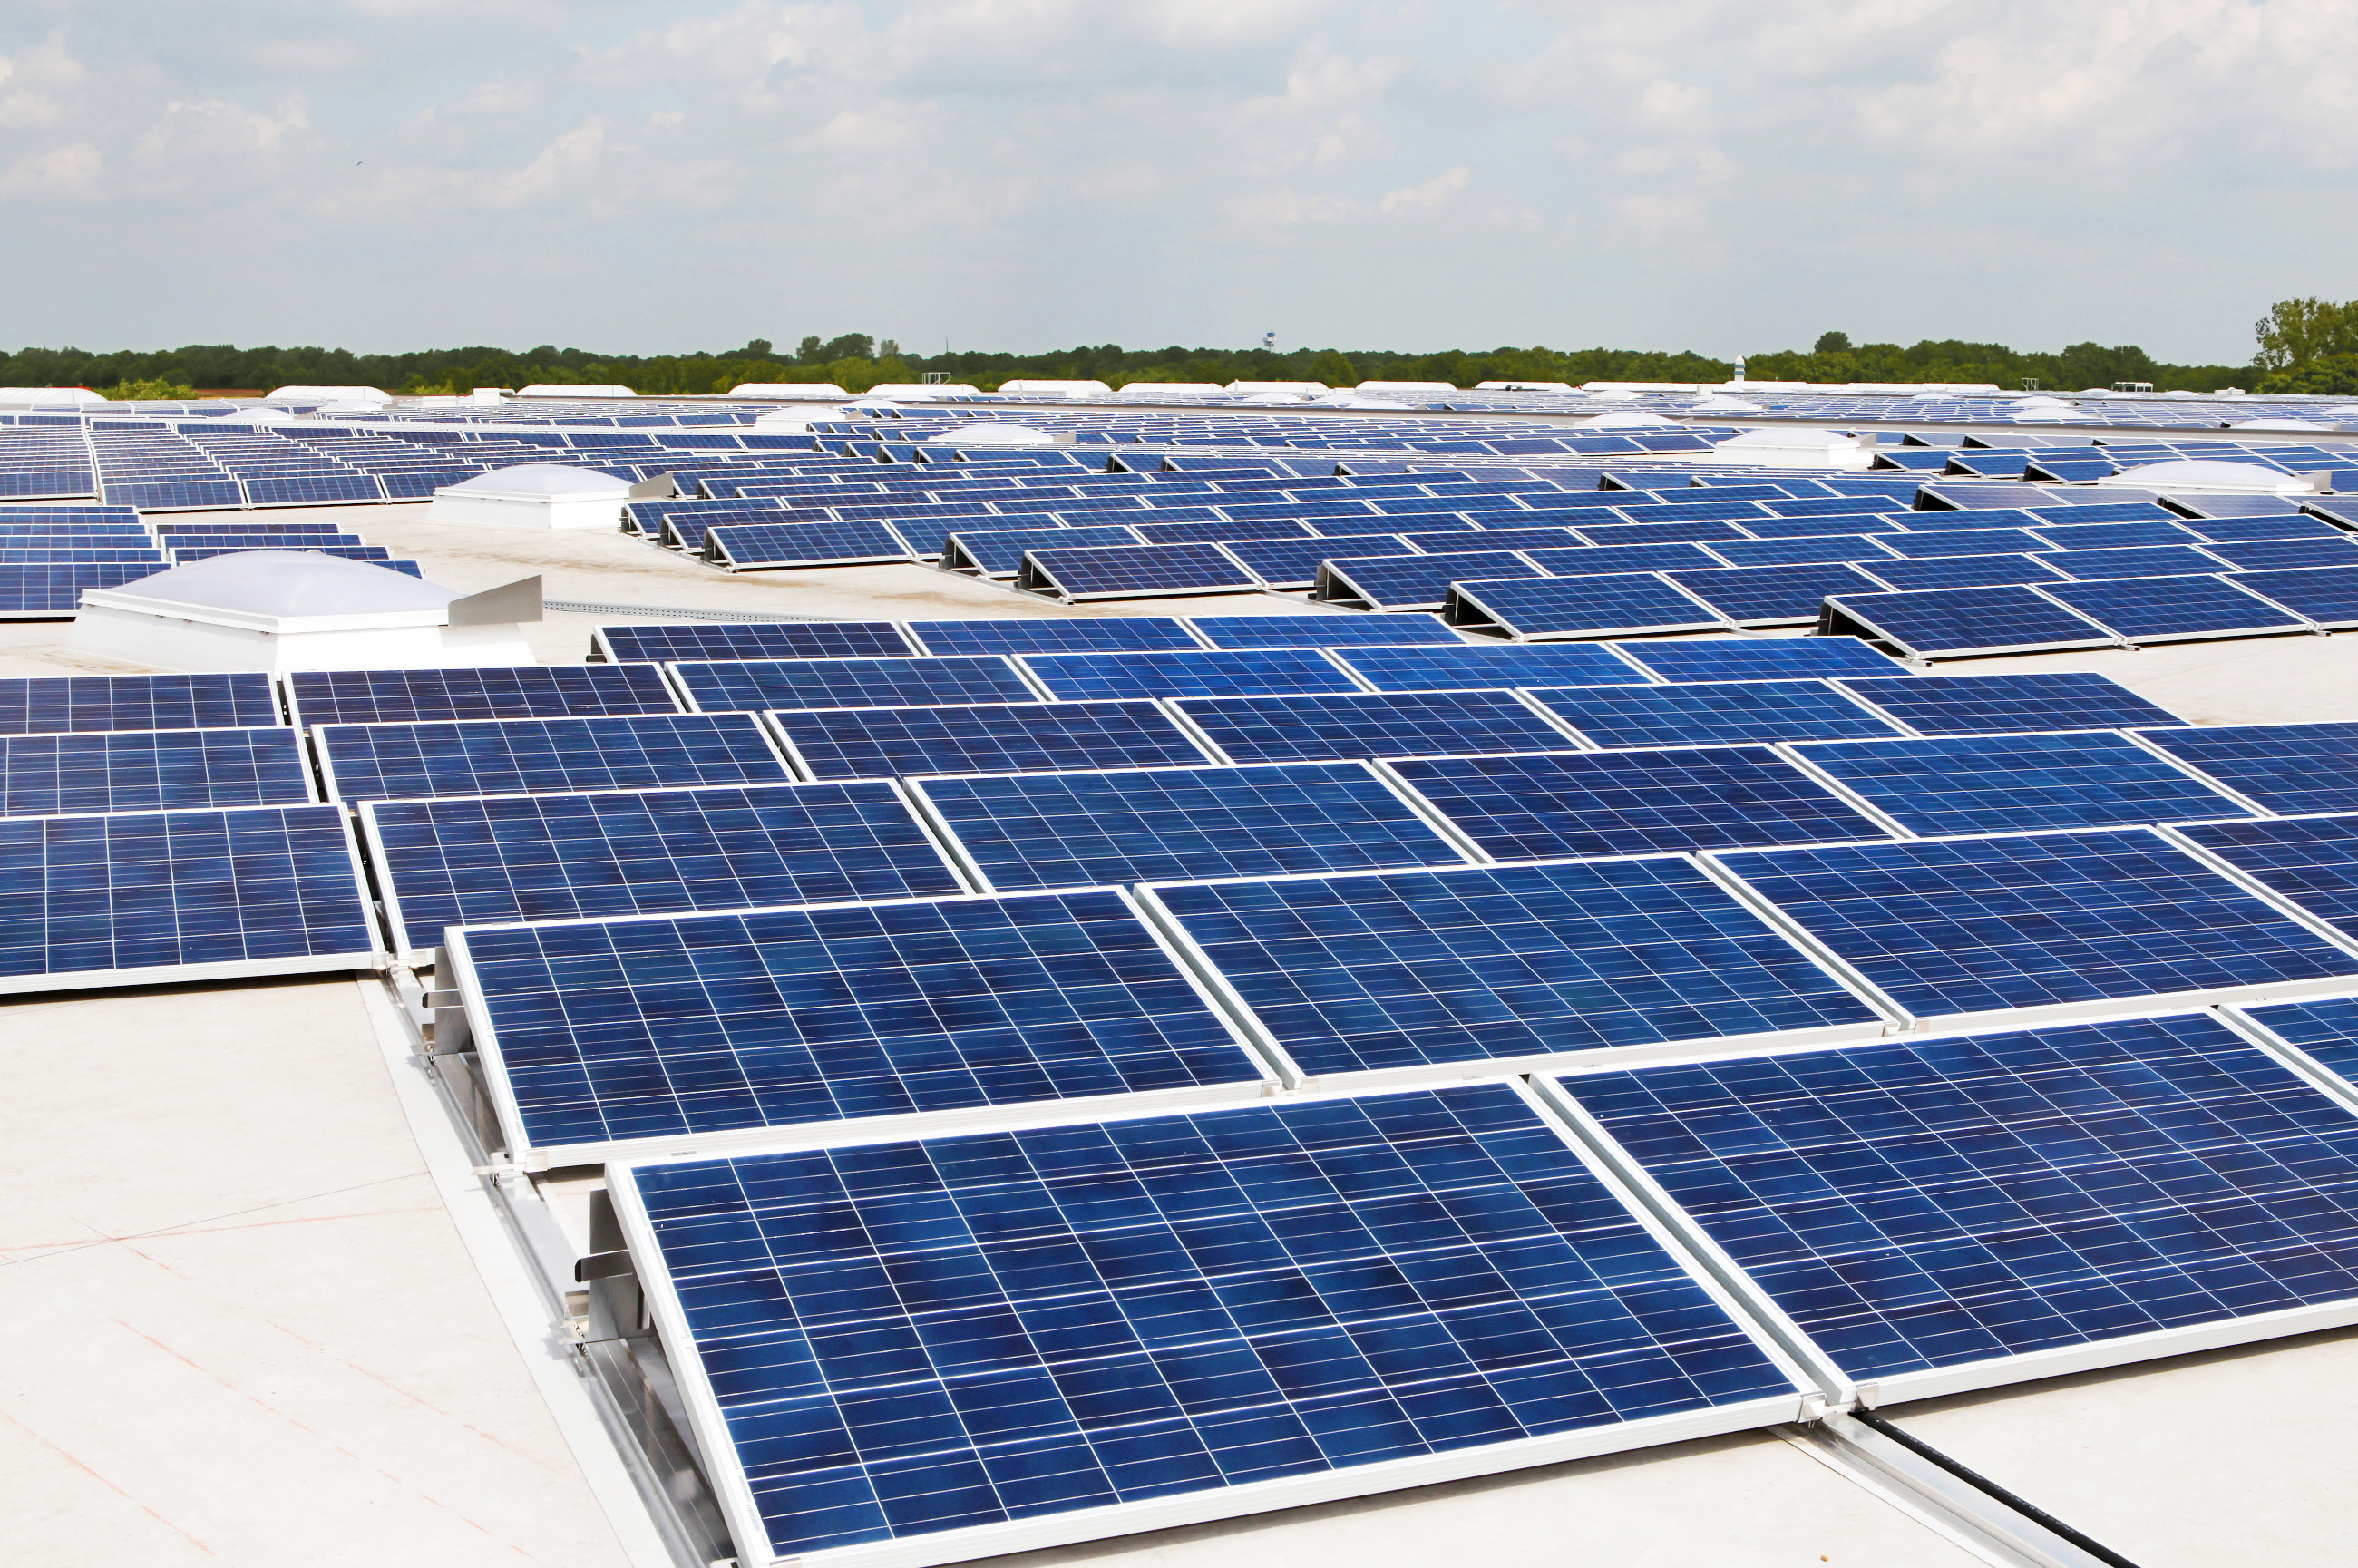
\includegraphics[width=\paperwidth,height=\paperheight]{images/titlepage/titlepic.jpg}%
        };
        %\node[
        %    fill=white,
        %    fill opacity=0.5,
        %    inner sep=0pt,
        %    anchor=west
        %] at (-38.5mm,-105mm) {%
        %    %% Creator: Matplotlib, PGF backend
%%
%% To include the figure in your LaTeX document, write
%%   \input{<filename>.pgf}
%%
%% Make sure the required packages are loaded in your preamble
%%   \usepackage{pgf}
%%
%% Figures using additional raster images can only be included by \input if
%% they are in the same directory as the main LaTeX file. For loading figures
%% from other directories you can use the `import` package
%%   \usepackage{import}
%% and then include the figures with
%%   \import{<path to file>}{<filename>.pgf}
%%
%% Matplotlib used the following preamble
%%   \usepackage{fontspec}
%%   \setmainfont{Bitstream Vera Serif}
%%   \setsansfont{Bitstream Vera Sans}
%%   \setmonofont{Bitstream Vera Sans Mono}
%%
\begingroup%
\makeatletter%
\begin{pgfpicture}%
\pgfpathrectangle{\pgfpointorigin}{\pgfqpoint{8.267700in}{2.000000in}}%
\pgfusepath{use as bounding box, clip}%
\begin{pgfscope}%
\pgfsetbuttcap%
\pgfsetmiterjoin%
\pgfsetlinewidth{0.000000pt}%
\definecolor{currentstroke}{rgb}{0.000000,0.000000,0.000000}%
\pgfsetstrokecolor{currentstroke}%
\pgfsetstrokeopacity{0.000000}%
\pgfsetdash{}{0pt}%
\pgfpathmoveto{\pgfqpoint{0.000000in}{0.000000in}}%
\pgfpathlineto{\pgfqpoint{8.267700in}{0.000000in}}%
\pgfpathlineto{\pgfqpoint{8.267700in}{2.000000in}}%
\pgfpathlineto{\pgfqpoint{0.000000in}{2.000000in}}%
\pgfpathclose%
\pgfusepath{}%
\end{pgfscope}%
\begin{pgfscope}%
\pgfsetbuttcap%
\pgfsetmiterjoin%
\pgfsetlinewidth{0.000000pt}%
\definecolor{currentstroke}{rgb}{0.000000,0.000000,0.000000}%
\pgfsetstrokecolor{currentstroke}%
\pgfsetstrokeopacity{0.000000}%
\pgfsetdash{}{0pt}%
\pgfpathmoveto{\pgfqpoint{0.826770in}{0.100000in}}%
\pgfpathlineto{\pgfqpoint{7.440930in}{0.100000in}}%
\pgfpathlineto{\pgfqpoint{7.440930in}{1.900000in}}%
\pgfpathlineto{\pgfqpoint{0.826770in}{1.900000in}}%
\pgfpathclose%
\pgfusepath{}%
\end{pgfscope}%
\begin{pgfscope}%
\pgfpathrectangle{\pgfqpoint{0.826770in}{0.100000in}}{\pgfqpoint{6.614160in}{1.800000in}} %
\pgfusepath{clip}%
\pgfsetroundcap%
\pgfsetroundjoin%
\pgfsetlinewidth{6.022500pt}%
\definecolor{currentstroke}{rgb}{0.500000,0.000000,0.000000}%
\pgfsetstrokecolor{currentstroke}%
\pgfsetdash{}{0pt}%
\pgfpathmoveto{\pgfqpoint{1.299210in}{1.000000in}}%
\pgfpathlineto{\pgfqpoint{1.333260in}{1.059662in}}%
\pgfpathlineto{\pgfqpoint{1.352176in}{1.088308in}}%
\pgfpathlineto{\pgfqpoint{1.367309in}{1.107297in}}%
\pgfpathlineto{\pgfqpoint{1.380551in}{1.120382in}}%
\pgfpathlineto{\pgfqpoint{1.391901in}{1.128645in}}%
\pgfpathlineto{\pgfqpoint{1.403251in}{1.133983in}}%
\pgfpathlineto{\pgfqpoint{1.412709in}{1.136107in}}%
\pgfpathlineto{\pgfqpoint{1.422167in}{1.136080in}}%
\pgfpathlineto{\pgfqpoint{1.431626in}{1.133903in}}%
\pgfpathlineto{\pgfqpoint{1.441084in}{1.129610in}}%
\pgfpathlineto{\pgfqpoint{1.452434in}{1.121763in}}%
\pgfpathlineto{\pgfqpoint{1.463784in}{1.111146in}}%
\pgfpathlineto{\pgfqpoint{1.477025in}{1.095586in}}%
\pgfpathlineto{\pgfqpoint{1.492158in}{1.074215in}}%
\pgfpathlineto{\pgfqpoint{1.511075in}{1.043401in}}%
\pgfpathlineto{\pgfqpoint{1.545125in}{0.982467in}}%
\pgfpathlineto{\pgfqpoint{1.571608in}{0.936892in}}%
\pgfpathlineto{\pgfqpoint{1.588633in}{0.911366in}}%
\pgfpathlineto{\pgfqpoint{1.603766in}{0.892438in}}%
\pgfpathlineto{\pgfqpoint{1.617007in}{0.879417in}}%
\pgfpathlineto{\pgfqpoint{1.628357in}{0.871213in}}%
\pgfpathlineto{\pgfqpoint{1.639707in}{0.865937in}}%
\pgfpathlineto{\pgfqpoint{1.649166in}{0.863867in}}%
\pgfpathlineto{\pgfqpoint{1.658624in}{0.863948in}}%
\pgfpathlineto{\pgfqpoint{1.668082in}{0.866179in}}%
\pgfpathlineto{\pgfqpoint{1.677540in}{0.870524in}}%
\pgfpathlineto{\pgfqpoint{1.688890in}{0.878431in}}%
\pgfpathlineto{\pgfqpoint{1.700240in}{0.889103in}}%
\pgfpathlineto{\pgfqpoint{1.713482in}{0.904720in}}%
\pgfpathlineto{\pgfqpoint{1.728615in}{0.926145in}}%
\pgfpathlineto{\pgfqpoint{1.747531in}{0.957006in}}%
\pgfpathlineto{\pgfqpoint{1.781581in}{1.017958in}}%
\pgfpathlineto{\pgfqpoint{1.808064in}{1.063488in}}%
\pgfpathlineto{\pgfqpoint{1.825089in}{1.088960in}}%
\pgfpathlineto{\pgfqpoint{1.840222in}{1.107825in}}%
\pgfpathlineto{\pgfqpoint{1.853464in}{1.120782in}}%
\pgfpathlineto{\pgfqpoint{1.864814in}{1.128927in}}%
\pgfpathlineto{\pgfqpoint{1.876164in}{1.134140in}}%
\pgfpathlineto{\pgfqpoint{1.885622in}{1.136157in}}%
\pgfpathlineto{\pgfqpoint{1.895080in}{1.136022in}}%
\pgfpathlineto{\pgfqpoint{1.904539in}{1.133738in}}%
\pgfpathlineto{\pgfqpoint{1.913997in}{1.129341in}}%
\pgfpathlineto{\pgfqpoint{1.925347in}{1.121374in}}%
\pgfpathlineto{\pgfqpoint{1.936697in}{1.110647in}}%
\pgfpathlineto{\pgfqpoint{1.949938in}{1.094973in}}%
\pgfpathlineto{\pgfqpoint{1.965071in}{1.073494in}}%
\pgfpathlineto{\pgfqpoint{1.983988in}{1.042587in}}%
\pgfpathlineto{\pgfqpoint{2.019929in}{0.978223in}}%
\pgfpathlineto{\pgfqpoint{2.046412in}{0.933122in}}%
\pgfpathlineto{\pgfqpoint{2.063437in}{0.908151in}}%
\pgfpathlineto{\pgfqpoint{2.078570in}{0.889856in}}%
\pgfpathlineto{\pgfqpoint{2.091812in}{0.877475in}}%
\pgfpathlineto{\pgfqpoint{2.103162in}{0.869867in}}%
\pgfpathlineto{\pgfqpoint{2.112620in}{0.865783in}}%
\pgfpathlineto{\pgfqpoint{2.122078in}{0.863820in}}%
\pgfpathlineto{\pgfqpoint{2.131537in}{0.864009in}}%
\pgfpathlineto{\pgfqpoint{2.140995in}{0.866346in}}%
\pgfpathlineto{\pgfqpoint{2.150453in}{0.870796in}}%
\pgfpathlineto{\pgfqpoint{2.161803in}{0.878822in}}%
\pgfpathlineto{\pgfqpoint{2.173153in}{0.889604in}}%
\pgfpathlineto{\pgfqpoint{2.186395in}{0.905336in}}%
\pgfpathlineto{\pgfqpoint{2.201528in}{0.926868in}}%
\pgfpathlineto{\pgfqpoint{2.220444in}{0.957821in}}%
\pgfpathlineto{\pgfqpoint{2.256386in}{1.022200in}}%
\pgfpathlineto{\pgfqpoint{2.282869in}{1.067251in}}%
\pgfpathlineto{\pgfqpoint{2.299894in}{1.092165in}}%
\pgfpathlineto{\pgfqpoint{2.315027in}{1.110396in}}%
\pgfpathlineto{\pgfqpoint{2.328268in}{1.122713in}}%
\pgfpathlineto{\pgfqpoint{2.339618in}{1.130260in}}%
\pgfpathlineto{\pgfqpoint{2.349077in}{1.134292in}}%
\pgfpathlineto{\pgfqpoint{2.358535in}{1.136202in}}%
\pgfpathlineto{\pgfqpoint{2.367993in}{1.135959in}}%
\pgfpathlineto{\pgfqpoint{2.377451in}{1.133568in}}%
\pgfpathlineto{\pgfqpoint{2.386910in}{1.129066in}}%
\pgfpathlineto{\pgfqpoint{2.398260in}{1.120981in}}%
\pgfpathlineto{\pgfqpoint{2.409610in}{1.110144in}}%
\pgfpathlineto{\pgfqpoint{2.422851in}{1.094355in}}%
\pgfpathlineto{\pgfqpoint{2.437984in}{1.072770in}}%
\pgfpathlineto{\pgfqpoint{2.456901in}{1.041771in}}%
\pgfpathlineto{\pgfqpoint{2.494734in}{0.974002in}}%
\pgfpathlineto{\pgfqpoint{2.519325in}{0.932376in}}%
\pgfpathlineto{\pgfqpoint{2.536350in}{0.907519in}}%
\pgfpathlineto{\pgfqpoint{2.551483in}{0.889353in}}%
\pgfpathlineto{\pgfqpoint{2.564725in}{0.877101in}}%
\pgfpathlineto{\pgfqpoint{2.576075in}{0.869614in}}%
\pgfpathlineto{\pgfqpoint{2.585533in}{0.865634in}}%
\pgfpathlineto{\pgfqpoint{2.594991in}{0.863778in}}%
\pgfpathlineto{\pgfqpoint{2.604450in}{0.864075in}}%
\pgfpathlineto{\pgfqpoint{2.613908in}{0.866519in}}%
\pgfpathlineto{\pgfqpoint{2.623366in}{0.871073in}}%
\pgfpathlineto{\pgfqpoint{2.634716in}{0.879218in}}%
\pgfpathlineto{\pgfqpoint{2.646066in}{0.890110in}}%
\pgfpathlineto{\pgfqpoint{2.659308in}{0.905955in}}%
\pgfpathlineto{\pgfqpoint{2.674441in}{0.927593in}}%
\pgfpathlineto{\pgfqpoint{2.693357in}{0.958637in}}%
\pgfpathlineto{\pgfqpoint{2.733082in}{1.029776in}}%
\pgfpathlineto{\pgfqpoint{2.757673in}{1.070948in}}%
\pgfpathlineto{\pgfqpoint{2.774698in}{1.095280in}}%
\pgfpathlineto{\pgfqpoint{2.787940in}{1.110897in}}%
\pgfpathlineto{\pgfqpoint{2.801181in}{1.123084in}}%
\pgfpathlineto{\pgfqpoint{2.812531in}{1.130511in}}%
\pgfpathlineto{\pgfqpoint{2.821990in}{1.134438in}}%
\pgfpathlineto{\pgfqpoint{2.831448in}{1.136241in}}%
\pgfpathlineto{\pgfqpoint{2.840906in}{1.135890in}}%
\pgfpathlineto{\pgfqpoint{2.850364in}{1.133393in}}%
\pgfpathlineto{\pgfqpoint{2.859823in}{1.128787in}}%
\pgfpathlineto{\pgfqpoint{2.871173in}{1.120583in}}%
\pgfpathlineto{\pgfqpoint{2.882522in}{1.109636in}}%
\pgfpathlineto{\pgfqpoint{2.895764in}{1.093734in}}%
\pgfpathlineto{\pgfqpoint{2.910897in}{1.072043in}}%
\pgfpathlineto{\pgfqpoint{2.929814in}{1.040954in}}%
\pgfpathlineto{\pgfqpoint{2.971430in}{0.966470in}}%
\pgfpathlineto{\pgfqpoint{2.994130in}{0.928686in}}%
\pgfpathlineto{\pgfqpoint{3.011155in}{0.904414in}}%
\pgfpathlineto{\pgfqpoint{3.024396in}{0.888854in}}%
\pgfpathlineto{\pgfqpoint{3.037638in}{0.876732in}}%
\pgfpathlineto{\pgfqpoint{3.048988in}{0.869365in}}%
\pgfpathlineto{\pgfqpoint{3.058446in}{0.865491in}}%
\pgfpathlineto{\pgfqpoint{3.067904in}{0.863742in}}%
\pgfpathlineto{\pgfqpoint{3.077363in}{0.864146in}}%
\pgfpathlineto{\pgfqpoint{3.086821in}{0.866697in}}%
\pgfpathlineto{\pgfqpoint{3.096279in}{0.871355in}}%
\pgfpathlineto{\pgfqpoint{3.107629in}{0.879618in}}%
\pgfpathlineto{\pgfqpoint{3.118979in}{0.890620in}}%
\pgfpathlineto{\pgfqpoint{3.132220in}{0.906578in}}%
\pgfpathlineto{\pgfqpoint{3.147354in}{0.928321in}}%
\pgfpathlineto{\pgfqpoint{3.166270in}{0.959455in}}%
\pgfpathlineto{\pgfqpoint{3.188970in}{1.000000in}}%
\pgfpathlineto{\pgfqpoint{3.188970in}{1.000000in}}%
\pgfusepath{stroke}%
\end{pgfscope}%
\begin{pgfscope}%
\pgfpathrectangle{\pgfqpoint{0.826770in}{0.100000in}}{\pgfqpoint{6.614160in}{1.800000in}} %
\pgfusepath{clip}%
\pgfsetroundcap%
\pgfsetroundjoin%
\pgfsetlinewidth{6.022500pt}%
\definecolor{currentstroke}{rgb}{0.500000,0.000000,0.000000}%
\pgfsetstrokecolor{currentstroke}%
\pgfsetdash{}{0pt}%
\pgfpathmoveto{\pgfqpoint{3.188970in}{1.000000in}}%
\pgfpathlineto{\pgfqpoint{3.221128in}{1.339353in}}%
\pgfpathlineto{\pgfqpoint{3.238153in}{1.497822in}}%
\pgfpathlineto{\pgfqpoint{3.251395in}{1.603878in}}%
\pgfpathlineto{\pgfqpoint{3.262744in}{1.680025in}}%
\pgfpathlineto{\pgfqpoint{3.272203in}{1.731730in}}%
\pgfpathlineto{\pgfqpoint{3.281661in}{1.771873in}}%
\pgfpathlineto{\pgfqpoint{3.289228in}{1.795229in}}%
\pgfpathlineto{\pgfqpoint{3.294902in}{1.807475in}}%
\pgfpathlineto{\pgfqpoint{3.300577in}{1.815124in}}%
\pgfpathlineto{\pgfqpoint{3.304361in}{1.817647in}}%
\pgfpathlineto{\pgfqpoint{3.308144in}{1.818100in}}%
\pgfpathlineto{\pgfqpoint{3.311927in}{1.816482in}}%
\pgfpathlineto{\pgfqpoint{3.315711in}{1.812798in}}%
\pgfpathlineto{\pgfqpoint{3.321386in}{1.803418in}}%
\pgfpathlineto{\pgfqpoint{3.327061in}{1.789464in}}%
\pgfpathlineto{\pgfqpoint{3.334627in}{1.763885in}}%
\pgfpathlineto{\pgfqpoint{3.342194in}{1.730576in}}%
\pgfpathlineto{\pgfqpoint{3.351652in}{1.678591in}}%
\pgfpathlineto{\pgfqpoint{3.363002in}{1.602139in}}%
\pgfpathlineto{\pgfqpoint{3.376244in}{1.495778in}}%
\pgfpathlineto{\pgfqpoint{3.391377in}{1.355658in}}%
\pgfpathlineto{\pgfqpoint{3.412185in}{1.140809in}}%
\pgfpathlineto{\pgfqpoint{3.463259in}{0.603225in}}%
\pgfpathlineto{\pgfqpoint{3.480284in}{0.452721in}}%
\pgfpathlineto{\pgfqpoint{3.493526in}{0.354631in}}%
\pgfpathlineto{\pgfqpoint{3.504876in}{0.286344in}}%
\pgfpathlineto{\pgfqpoint{3.514334in}{0.241781in}}%
\pgfpathlineto{\pgfqpoint{3.521901in}{0.214730in}}%
\pgfpathlineto{\pgfqpoint{3.529467in}{0.195624in}}%
\pgfpathlineto{\pgfqpoint{3.535142in}{0.186629in}}%
\pgfpathlineto{\pgfqpoint{3.540817in}{0.182264in}}%
\pgfpathlineto{\pgfqpoint{3.544601in}{0.181941in}}%
\pgfpathlineto{\pgfqpoint{3.548384in}{0.183688in}}%
\pgfpathlineto{\pgfqpoint{3.552167in}{0.187501in}}%
\pgfpathlineto{\pgfqpoint{3.557842in}{0.197072in}}%
\pgfpathlineto{\pgfqpoint{3.563517in}{0.211215in}}%
\pgfpathlineto{\pgfqpoint{3.571084in}{0.237041in}}%
\pgfpathlineto{\pgfqpoint{3.578650in}{0.270586in}}%
\pgfpathlineto{\pgfqpoint{3.588108in}{0.322850in}}%
\pgfpathlineto{\pgfqpoint{3.599458in}{0.399606in}}%
\pgfpathlineto{\pgfqpoint{3.612700in}{0.506271in}}%
\pgfpathlineto{\pgfqpoint{3.627833in}{0.646661in}}%
\pgfpathlineto{\pgfqpoint{3.648641in}{0.861727in}}%
\pgfpathlineto{\pgfqpoint{3.699716in}{1.399023in}}%
\pgfpathlineto{\pgfqpoint{3.716741in}{1.549189in}}%
\pgfpathlineto{\pgfqpoint{3.729982in}{1.646948in}}%
\pgfpathlineto{\pgfqpoint{3.741332in}{1.714911in}}%
\pgfpathlineto{\pgfqpoint{3.750791in}{1.759182in}}%
\pgfpathlineto{\pgfqpoint{3.758357in}{1.785988in}}%
\pgfpathlineto{\pgfqpoint{3.765924in}{1.804842in}}%
\pgfpathlineto{\pgfqpoint{3.771599in}{1.813646in}}%
\pgfpathlineto{\pgfqpoint{3.777274in}{1.817817in}}%
\pgfpathlineto{\pgfqpoint{3.781057in}{1.818011in}}%
\pgfpathlineto{\pgfqpoint{3.784840in}{1.816135in}}%
\pgfpathlineto{\pgfqpoint{3.788624in}{1.812192in}}%
\pgfpathlineto{\pgfqpoint{3.794299in}{1.802429in}}%
\pgfpathlineto{\pgfqpoint{3.799973in}{1.788097in}}%
\pgfpathlineto{\pgfqpoint{3.807540in}{1.762026in}}%
\pgfpathlineto{\pgfqpoint{3.815107in}{1.728245in}}%
\pgfpathlineto{\pgfqpoint{3.824565in}{1.675703in}}%
\pgfpathlineto{\pgfqpoint{3.835915in}{1.598643in}}%
\pgfpathlineto{\pgfqpoint{3.849156in}{1.491675in}}%
\pgfpathlineto{\pgfqpoint{3.864290in}{1.351017in}}%
\pgfpathlineto{\pgfqpoint{3.885098in}{1.135737in}}%
\pgfpathlineto{\pgfqpoint{3.934281in}{0.616796in}}%
\pgfpathlineto{\pgfqpoint{3.951306in}{0.464293in}}%
\pgfpathlineto{\pgfqpoint{3.964547in}{0.364234in}}%
\pgfpathlineto{\pgfqpoint{3.975897in}{0.294021in}}%
\pgfpathlineto{\pgfqpoint{3.985355in}{0.247717in}}%
\pgfpathlineto{\pgfqpoint{3.992922in}{0.219204in}}%
\pgfpathlineto{\pgfqpoint{4.000489in}{0.198591in}}%
\pgfpathlineto{\pgfqpoint{4.006164in}{0.188445in}}%
\pgfpathlineto{\pgfqpoint{4.011838in}{0.182919in}}%
\pgfpathlineto{\pgfqpoint{4.015622in}{0.181819in}}%
\pgfpathlineto{\pgfqpoint{4.019405in}{0.182790in}}%
\pgfpathlineto{\pgfqpoint{4.023188in}{0.185829in}}%
\pgfpathlineto{\pgfqpoint{4.028863in}{0.194248in}}%
\pgfpathlineto{\pgfqpoint{4.034538in}{0.207255in}}%
\pgfpathlineto{\pgfqpoint{4.042105in}{0.231602in}}%
\pgfpathlineto{\pgfqpoint{4.049672in}{0.263723in}}%
\pgfpathlineto{\pgfqpoint{4.059130in}{0.314306in}}%
\pgfpathlineto{\pgfqpoint{4.070480in}{0.389225in}}%
\pgfpathlineto{\pgfqpoint{4.083721in}{0.494050in}}%
\pgfpathlineto{\pgfqpoint{4.098854in}{0.632801in}}%
\pgfpathlineto{\pgfqpoint{4.119663in}{0.846536in}}%
\pgfpathlineto{\pgfqpoint{4.172629in}{1.403508in}}%
\pgfpathlineto{\pgfqpoint{4.187762in}{1.537649in}}%
\pgfpathlineto{\pgfqpoint{4.201004in}{1.637382in}}%
\pgfpathlineto{\pgfqpoint{4.212354in}{1.707276in}}%
\pgfpathlineto{\pgfqpoint{4.221812in}{1.753291in}}%
\pgfpathlineto{\pgfqpoint{4.229378in}{1.781561in}}%
\pgfpathlineto{\pgfqpoint{4.236945in}{1.801923in}}%
\pgfpathlineto{\pgfqpoint{4.242620in}{1.811878in}}%
\pgfpathlineto{\pgfqpoint{4.248295in}{1.817210in}}%
\pgfpathlineto{\pgfqpoint{4.252078in}{1.818181in}}%
\pgfpathlineto{\pgfqpoint{4.255862in}{1.817081in}}%
\pgfpathlineto{\pgfqpoint{4.259645in}{1.813912in}}%
\pgfpathlineto{\pgfqpoint{4.265320in}{1.805301in}}%
\pgfpathlineto{\pgfqpoint{4.270995in}{1.792105in}}%
\pgfpathlineto{\pgfqpoint{4.278561in}{1.767511in}}%
\pgfpathlineto{\pgfqpoint{4.286128in}{1.735151in}}%
\pgfpathlineto{\pgfqpoint{4.295586in}{1.684287in}}%
\pgfpathlineto{\pgfqpoint{4.306936in}{1.609059in}}%
\pgfpathlineto{\pgfqpoint{4.320178in}{1.503926in}}%
\pgfpathlineto{\pgfqpoint{4.335311in}{1.364898in}}%
\pgfpathlineto{\pgfqpoint{4.356119in}{1.150936in}}%
\pgfpathlineto{\pgfqpoint{4.409085in}{0.594256in}}%
\pgfpathlineto{\pgfqpoint{4.424219in}{0.460414in}}%
\pgfpathlineto{\pgfqpoint{4.437460in}{0.361008in}}%
\pgfpathlineto{\pgfqpoint{4.448810in}{0.291434in}}%
\pgfpathlineto{\pgfqpoint{4.458268in}{0.245708in}}%
\pgfpathlineto{\pgfqpoint{4.465835in}{0.217682in}}%
\pgfpathlineto{\pgfqpoint{4.473401in}{0.197571in}}%
\pgfpathlineto{\pgfqpoint{4.479076in}{0.187808in}}%
\pgfpathlineto{\pgfqpoint{4.484751in}{0.182669in}}%
\pgfpathlineto{\pgfqpoint{4.488535in}{0.181827in}}%
\pgfpathlineto{\pgfqpoint{4.492318in}{0.183057in}}%
\pgfpathlineto{\pgfqpoint{4.496101in}{0.186354in}}%
\pgfpathlineto{\pgfqpoint{4.501776in}{0.195158in}}%
\pgfpathlineto{\pgfqpoint{4.507451in}{0.208544in}}%
\pgfpathlineto{\pgfqpoint{4.515018in}{0.233384in}}%
\pgfpathlineto{\pgfqpoint{4.522584in}{0.265982in}}%
\pgfpathlineto{\pgfqpoint{4.532043in}{0.317127in}}%
\pgfpathlineto{\pgfqpoint{4.543393in}{0.392662in}}%
\pgfpathlineto{\pgfqpoint{4.556634in}{0.498104in}}%
\pgfpathlineto{\pgfqpoint{4.571767in}{0.637406in}}%
\pgfpathlineto{\pgfqpoint{4.592576in}{0.851594in}}%
\pgfpathlineto{\pgfqpoint{4.645542in}{1.407976in}}%
\pgfpathlineto{\pgfqpoint{4.660675in}{1.541517in}}%
\pgfpathlineto{\pgfqpoint{4.673917in}{1.640596in}}%
\pgfpathlineto{\pgfqpoint{4.685266in}{1.709849in}}%
\pgfpathlineto{\pgfqpoint{4.694725in}{1.755285in}}%
\pgfpathlineto{\pgfqpoint{4.702291in}{1.783068in}}%
\pgfpathlineto{\pgfqpoint{4.709858in}{1.802928in}}%
\pgfpathlineto{\pgfqpoint{4.715533in}{1.812499in}}%
\pgfpathlineto{\pgfqpoint{4.721208in}{1.817445in}}%
\pgfpathlineto{\pgfqpoint{4.724991in}{1.818157in}}%
\pgfpathlineto{\pgfqpoint{4.728774in}{1.816798in}}%
\pgfpathlineto{\pgfqpoint{4.732558in}{1.813371in}}%
\pgfpathlineto{\pgfqpoint{4.738233in}{1.804376in}}%
\pgfpathlineto{\pgfqpoint{4.743908in}{1.790800in}}%
\pgfpathlineto{\pgfqpoint{4.751474in}{1.765713in}}%
\pgfpathlineto{\pgfqpoint{4.759041in}{1.732878in}}%
\pgfpathlineto{\pgfqpoint{4.768499in}{1.681453in}}%
\pgfpathlineto{\pgfqpoint{4.779849in}{1.605611in}}%
\pgfpathlineto{\pgfqpoint{4.793091in}{1.499862in}}%
\pgfpathlineto{\pgfqpoint{4.808224in}{1.360285in}}%
\pgfpathlineto{\pgfqpoint{4.829032in}{1.145875in}}%
\pgfpathlineto{\pgfqpoint{4.880107in}{0.607733in}}%
\pgfpathlineto{\pgfqpoint{4.897131in}{0.456557in}}%
\pgfpathlineto{\pgfqpoint{4.910373in}{0.357807in}}%
\pgfpathlineto{\pgfqpoint{4.921723in}{0.288875in}}%
\pgfpathlineto{\pgfqpoint{4.931181in}{0.243730in}}%
\pgfpathlineto{\pgfqpoint{4.938748in}{0.216190in}}%
\pgfpathlineto{\pgfqpoint{4.946314in}{0.196582in}}%
\pgfpathlineto{\pgfqpoint{4.951989in}{0.187202in}}%
\pgfpathlineto{\pgfqpoint{4.957664in}{0.182450in}}%
\pgfpathlineto{\pgfqpoint{4.961448in}{0.181868in}}%
\pgfpathlineto{\pgfqpoint{4.965231in}{0.183356in}}%
\pgfpathlineto{\pgfqpoint{4.969014in}{0.186911in}}%
\pgfpathlineto{\pgfqpoint{4.974689in}{0.196099in}}%
\pgfpathlineto{\pgfqpoint{4.980364in}{0.209864in}}%
\pgfpathlineto{\pgfqpoint{4.987931in}{0.235197in}}%
\pgfpathlineto{\pgfqpoint{4.995497in}{0.268270in}}%
\pgfpathlineto{\pgfqpoint{5.004956in}{0.319975in}}%
\pgfpathlineto{\pgfqpoint{5.016305in}{0.396122in}}%
\pgfpathlineto{\pgfqpoint{5.029547in}{0.502178in}}%
\pgfpathlineto{\pgfqpoint{5.044680in}{0.642027in}}%
\pgfpathlineto{\pgfqpoint{5.065488in}{0.856657in}}%
\pgfpathlineto{\pgfqpoint{5.078730in}{1.000000in}}%
\pgfpathlineto{\pgfqpoint{5.078730in}{1.000000in}}%
\pgfusepath{stroke}%
\end{pgfscope}%
\begin{pgfscope}%
\pgfpathrectangle{\pgfqpoint{0.826770in}{0.100000in}}{\pgfqpoint{6.614160in}{1.800000in}} %
\pgfusepath{clip}%
\pgfsetroundcap%
\pgfsetroundjoin%
\pgfsetlinewidth{6.022500pt}%
\definecolor{currentstroke}{rgb}{0.500000,0.000000,0.000000}%
\pgfsetstrokecolor{currentstroke}%
\pgfsetdash{}{0pt}%
\pgfpathmoveto{\pgfqpoint{5.078730in}{1.000000in}}%
\pgfpathlineto{\pgfqpoint{5.112780in}{1.059662in}}%
\pgfpathlineto{\pgfqpoint{5.131696in}{1.088308in}}%
\pgfpathlineto{\pgfqpoint{5.146829in}{1.107297in}}%
\pgfpathlineto{\pgfqpoint{5.160071in}{1.120382in}}%
\pgfpathlineto{\pgfqpoint{5.171421in}{1.128645in}}%
\pgfpathlineto{\pgfqpoint{5.182771in}{1.133983in}}%
\pgfpathlineto{\pgfqpoint{5.192229in}{1.136107in}}%
\pgfpathlineto{\pgfqpoint{5.201687in}{1.136080in}}%
\pgfpathlineto{\pgfqpoint{5.211146in}{1.133903in}}%
\pgfpathlineto{\pgfqpoint{5.220604in}{1.129610in}}%
\pgfpathlineto{\pgfqpoint{5.231954in}{1.121763in}}%
\pgfpathlineto{\pgfqpoint{5.243304in}{1.111146in}}%
\pgfpathlineto{\pgfqpoint{5.256545in}{1.095586in}}%
\pgfpathlineto{\pgfqpoint{5.271678in}{1.074215in}}%
\pgfpathlineto{\pgfqpoint{5.290595in}{1.043401in}}%
\pgfpathlineto{\pgfqpoint{5.324645in}{0.982467in}}%
\pgfpathlineto{\pgfqpoint{5.351128in}{0.936892in}}%
\pgfpathlineto{\pgfqpoint{5.368153in}{0.911366in}}%
\pgfpathlineto{\pgfqpoint{5.383286in}{0.892438in}}%
\pgfpathlineto{\pgfqpoint{5.396527in}{0.879417in}}%
\pgfpathlineto{\pgfqpoint{5.407877in}{0.871213in}}%
\pgfpathlineto{\pgfqpoint{5.419227in}{0.865937in}}%
\pgfpathlineto{\pgfqpoint{5.428686in}{0.863867in}}%
\pgfpathlineto{\pgfqpoint{5.438144in}{0.863948in}}%
\pgfpathlineto{\pgfqpoint{5.447602in}{0.866179in}}%
\pgfpathlineto{\pgfqpoint{5.457060in}{0.870524in}}%
\pgfpathlineto{\pgfqpoint{5.468410in}{0.878431in}}%
\pgfpathlineto{\pgfqpoint{5.479760in}{0.889103in}}%
\pgfpathlineto{\pgfqpoint{5.493002in}{0.904720in}}%
\pgfpathlineto{\pgfqpoint{5.508135in}{0.926145in}}%
\pgfpathlineto{\pgfqpoint{5.527051in}{0.957006in}}%
\pgfpathlineto{\pgfqpoint{5.561101in}{1.017958in}}%
\pgfpathlineto{\pgfqpoint{5.587584in}{1.063488in}}%
\pgfpathlineto{\pgfqpoint{5.604609in}{1.088960in}}%
\pgfpathlineto{\pgfqpoint{5.619742in}{1.107825in}}%
\pgfpathlineto{\pgfqpoint{5.632984in}{1.120782in}}%
\pgfpathlineto{\pgfqpoint{5.644334in}{1.128927in}}%
\pgfpathlineto{\pgfqpoint{5.655684in}{1.134140in}}%
\pgfpathlineto{\pgfqpoint{5.665142in}{1.136157in}}%
\pgfpathlineto{\pgfqpoint{5.674600in}{1.136022in}}%
\pgfpathlineto{\pgfqpoint{5.684059in}{1.133738in}}%
\pgfpathlineto{\pgfqpoint{5.693517in}{1.129341in}}%
\pgfpathlineto{\pgfqpoint{5.704867in}{1.121374in}}%
\pgfpathlineto{\pgfqpoint{5.716217in}{1.110647in}}%
\pgfpathlineto{\pgfqpoint{5.729458in}{1.094973in}}%
\pgfpathlineto{\pgfqpoint{5.744591in}{1.073494in}}%
\pgfpathlineto{\pgfqpoint{5.763508in}{1.042587in}}%
\pgfpathlineto{\pgfqpoint{5.799449in}{0.978223in}}%
\pgfpathlineto{\pgfqpoint{5.825932in}{0.933122in}}%
\pgfpathlineto{\pgfqpoint{5.842957in}{0.908151in}}%
\pgfpathlineto{\pgfqpoint{5.858090in}{0.889856in}}%
\pgfpathlineto{\pgfqpoint{5.871332in}{0.877475in}}%
\pgfpathlineto{\pgfqpoint{5.882682in}{0.869867in}}%
\pgfpathlineto{\pgfqpoint{5.892140in}{0.865783in}}%
\pgfpathlineto{\pgfqpoint{5.901598in}{0.863820in}}%
\pgfpathlineto{\pgfqpoint{5.911057in}{0.864009in}}%
\pgfpathlineto{\pgfqpoint{5.920515in}{0.866346in}}%
\pgfpathlineto{\pgfqpoint{5.929973in}{0.870796in}}%
\pgfpathlineto{\pgfqpoint{5.941323in}{0.878822in}}%
\pgfpathlineto{\pgfqpoint{5.952673in}{0.889604in}}%
\pgfpathlineto{\pgfqpoint{5.965915in}{0.905336in}}%
\pgfpathlineto{\pgfqpoint{5.981048in}{0.926868in}}%
\pgfpathlineto{\pgfqpoint{5.999964in}{0.957821in}}%
\pgfpathlineto{\pgfqpoint{6.035906in}{1.022200in}}%
\pgfpathlineto{\pgfqpoint{6.062389in}{1.067251in}}%
\pgfpathlineto{\pgfqpoint{6.079414in}{1.092165in}}%
\pgfpathlineto{\pgfqpoint{6.094547in}{1.110396in}}%
\pgfpathlineto{\pgfqpoint{6.107788in}{1.122713in}}%
\pgfpathlineto{\pgfqpoint{6.119138in}{1.130260in}}%
\pgfpathlineto{\pgfqpoint{6.128597in}{1.134292in}}%
\pgfpathlineto{\pgfqpoint{6.138055in}{1.136202in}}%
\pgfpathlineto{\pgfqpoint{6.147513in}{1.135959in}}%
\pgfpathlineto{\pgfqpoint{6.156971in}{1.133568in}}%
\pgfpathlineto{\pgfqpoint{6.166430in}{1.129066in}}%
\pgfpathlineto{\pgfqpoint{6.177780in}{1.120981in}}%
\pgfpathlineto{\pgfqpoint{6.189130in}{1.110144in}}%
\pgfpathlineto{\pgfqpoint{6.202371in}{1.094355in}}%
\pgfpathlineto{\pgfqpoint{6.217504in}{1.072770in}}%
\pgfpathlineto{\pgfqpoint{6.236421in}{1.041771in}}%
\pgfpathlineto{\pgfqpoint{6.274254in}{0.974002in}}%
\pgfpathlineto{\pgfqpoint{6.298845in}{0.932376in}}%
\pgfpathlineto{\pgfqpoint{6.315870in}{0.907519in}}%
\pgfpathlineto{\pgfqpoint{6.331003in}{0.889353in}}%
\pgfpathlineto{\pgfqpoint{6.344245in}{0.877101in}}%
\pgfpathlineto{\pgfqpoint{6.355595in}{0.869614in}}%
\pgfpathlineto{\pgfqpoint{6.365053in}{0.865634in}}%
\pgfpathlineto{\pgfqpoint{6.374511in}{0.863778in}}%
\pgfpathlineto{\pgfqpoint{6.383970in}{0.864075in}}%
\pgfpathlineto{\pgfqpoint{6.393428in}{0.866519in}}%
\pgfpathlineto{\pgfqpoint{6.402886in}{0.871073in}}%
\pgfpathlineto{\pgfqpoint{6.414236in}{0.879218in}}%
\pgfpathlineto{\pgfqpoint{6.425586in}{0.890110in}}%
\pgfpathlineto{\pgfqpoint{6.438828in}{0.905955in}}%
\pgfpathlineto{\pgfqpoint{6.453961in}{0.927593in}}%
\pgfpathlineto{\pgfqpoint{6.472877in}{0.958637in}}%
\pgfpathlineto{\pgfqpoint{6.512602in}{1.029776in}}%
\pgfpathlineto{\pgfqpoint{6.537193in}{1.070948in}}%
\pgfpathlineto{\pgfqpoint{6.554218in}{1.095280in}}%
\pgfpathlineto{\pgfqpoint{6.567460in}{1.110897in}}%
\pgfpathlineto{\pgfqpoint{6.580701in}{1.123084in}}%
\pgfpathlineto{\pgfqpoint{6.592051in}{1.130511in}}%
\pgfpathlineto{\pgfqpoint{6.601510in}{1.134438in}}%
\pgfpathlineto{\pgfqpoint{6.610968in}{1.136241in}}%
\pgfpathlineto{\pgfqpoint{6.620426in}{1.135890in}}%
\pgfpathlineto{\pgfqpoint{6.629884in}{1.133393in}}%
\pgfpathlineto{\pgfqpoint{6.639343in}{1.128787in}}%
\pgfpathlineto{\pgfqpoint{6.650693in}{1.120583in}}%
\pgfpathlineto{\pgfqpoint{6.662042in}{1.109636in}}%
\pgfpathlineto{\pgfqpoint{6.675284in}{1.093734in}}%
\pgfpathlineto{\pgfqpoint{6.690417in}{1.072043in}}%
\pgfpathlineto{\pgfqpoint{6.709334in}{1.040954in}}%
\pgfpathlineto{\pgfqpoint{6.750950in}{0.966470in}}%
\pgfpathlineto{\pgfqpoint{6.773650in}{0.928686in}}%
\pgfpathlineto{\pgfqpoint{6.790675in}{0.904414in}}%
\pgfpathlineto{\pgfqpoint{6.803916in}{0.888854in}}%
\pgfpathlineto{\pgfqpoint{6.817158in}{0.876732in}}%
\pgfpathlineto{\pgfqpoint{6.828508in}{0.869365in}}%
\pgfpathlineto{\pgfqpoint{6.837966in}{0.865491in}}%
\pgfpathlineto{\pgfqpoint{6.847424in}{0.863742in}}%
\pgfpathlineto{\pgfqpoint{6.856883in}{0.864146in}}%
\pgfpathlineto{\pgfqpoint{6.866341in}{0.866697in}}%
\pgfpathlineto{\pgfqpoint{6.875799in}{0.871355in}}%
\pgfpathlineto{\pgfqpoint{6.887149in}{0.879618in}}%
\pgfpathlineto{\pgfqpoint{6.898499in}{0.890620in}}%
\pgfpathlineto{\pgfqpoint{6.911740in}{0.906578in}}%
\pgfpathlineto{\pgfqpoint{6.926874in}{0.928321in}}%
\pgfpathlineto{\pgfqpoint{6.945790in}{0.959455in}}%
\pgfpathlineto{\pgfqpoint{6.968490in}{1.000000in}}%
\pgfpathlineto{\pgfqpoint{6.968490in}{1.000000in}}%
\pgfusepath{stroke}%
\end{pgfscope}%
\begin{pgfscope}%
\pgfpathrectangle{\pgfqpoint{0.826770in}{0.100000in}}{\pgfqpoint{6.614160in}{1.800000in}} %
\pgfusepath{clip}%
\pgfsetroundcap%
\pgfsetroundjoin%
\pgfsetlinewidth{4.015000pt}%
\definecolor{currentstroke}{rgb}{0.750000,0.000000,0.000000}%
\pgfsetstrokecolor{currentstroke}%
\pgfsetdash{}{0pt}%
\pgfpathmoveto{\pgfqpoint{1.299210in}{1.000000in}}%
\pgfpathlineto{\pgfqpoint{1.333260in}{1.059662in}}%
\pgfpathlineto{\pgfqpoint{1.352176in}{1.088308in}}%
\pgfpathlineto{\pgfqpoint{1.367309in}{1.107297in}}%
\pgfpathlineto{\pgfqpoint{1.380551in}{1.120382in}}%
\pgfpathlineto{\pgfqpoint{1.391901in}{1.128645in}}%
\pgfpathlineto{\pgfqpoint{1.403251in}{1.133983in}}%
\pgfpathlineto{\pgfqpoint{1.412709in}{1.136107in}}%
\pgfpathlineto{\pgfqpoint{1.422167in}{1.136080in}}%
\pgfpathlineto{\pgfqpoint{1.431626in}{1.133903in}}%
\pgfpathlineto{\pgfqpoint{1.441084in}{1.129610in}}%
\pgfpathlineto{\pgfqpoint{1.452434in}{1.121763in}}%
\pgfpathlineto{\pgfqpoint{1.463784in}{1.111146in}}%
\pgfpathlineto{\pgfqpoint{1.477025in}{1.095586in}}%
\pgfpathlineto{\pgfqpoint{1.492158in}{1.074215in}}%
\pgfpathlineto{\pgfqpoint{1.511075in}{1.043401in}}%
\pgfpathlineto{\pgfqpoint{1.545125in}{0.982467in}}%
\pgfpathlineto{\pgfqpoint{1.571608in}{0.936892in}}%
\pgfpathlineto{\pgfqpoint{1.588633in}{0.911366in}}%
\pgfpathlineto{\pgfqpoint{1.603766in}{0.892438in}}%
\pgfpathlineto{\pgfqpoint{1.617007in}{0.879417in}}%
\pgfpathlineto{\pgfqpoint{1.628357in}{0.871213in}}%
\pgfpathlineto{\pgfqpoint{1.639707in}{0.865937in}}%
\pgfpathlineto{\pgfqpoint{1.649166in}{0.863867in}}%
\pgfpathlineto{\pgfqpoint{1.658624in}{0.863948in}}%
\pgfpathlineto{\pgfqpoint{1.668082in}{0.866179in}}%
\pgfpathlineto{\pgfqpoint{1.677540in}{0.870524in}}%
\pgfpathlineto{\pgfqpoint{1.688890in}{0.878431in}}%
\pgfpathlineto{\pgfqpoint{1.700240in}{0.889103in}}%
\pgfpathlineto{\pgfqpoint{1.713482in}{0.904720in}}%
\pgfpathlineto{\pgfqpoint{1.728615in}{0.926145in}}%
\pgfpathlineto{\pgfqpoint{1.747531in}{0.957006in}}%
\pgfpathlineto{\pgfqpoint{1.781581in}{1.017958in}}%
\pgfpathlineto{\pgfqpoint{1.808064in}{1.063488in}}%
\pgfpathlineto{\pgfqpoint{1.825089in}{1.088960in}}%
\pgfpathlineto{\pgfqpoint{1.840222in}{1.107825in}}%
\pgfpathlineto{\pgfqpoint{1.853464in}{1.120782in}}%
\pgfpathlineto{\pgfqpoint{1.864814in}{1.128927in}}%
\pgfpathlineto{\pgfqpoint{1.876164in}{1.134140in}}%
\pgfpathlineto{\pgfqpoint{1.885622in}{1.136157in}}%
\pgfpathlineto{\pgfqpoint{1.895080in}{1.136022in}}%
\pgfpathlineto{\pgfqpoint{1.904539in}{1.133738in}}%
\pgfpathlineto{\pgfqpoint{1.913997in}{1.129341in}}%
\pgfpathlineto{\pgfqpoint{1.925347in}{1.121374in}}%
\pgfpathlineto{\pgfqpoint{1.936697in}{1.110647in}}%
\pgfpathlineto{\pgfqpoint{1.949938in}{1.094973in}}%
\pgfpathlineto{\pgfqpoint{1.965071in}{1.073494in}}%
\pgfpathlineto{\pgfqpoint{1.983988in}{1.042587in}}%
\pgfpathlineto{\pgfqpoint{2.019929in}{0.978223in}}%
\pgfpathlineto{\pgfqpoint{2.046412in}{0.933122in}}%
\pgfpathlineto{\pgfqpoint{2.063437in}{0.908151in}}%
\pgfpathlineto{\pgfqpoint{2.078570in}{0.889856in}}%
\pgfpathlineto{\pgfqpoint{2.091812in}{0.877475in}}%
\pgfpathlineto{\pgfqpoint{2.103162in}{0.869867in}}%
\pgfpathlineto{\pgfqpoint{2.112620in}{0.865783in}}%
\pgfpathlineto{\pgfqpoint{2.122078in}{0.863820in}}%
\pgfpathlineto{\pgfqpoint{2.131537in}{0.864009in}}%
\pgfpathlineto{\pgfqpoint{2.140995in}{0.866346in}}%
\pgfpathlineto{\pgfqpoint{2.150453in}{0.870796in}}%
\pgfpathlineto{\pgfqpoint{2.161803in}{0.878822in}}%
\pgfpathlineto{\pgfqpoint{2.173153in}{0.889604in}}%
\pgfpathlineto{\pgfqpoint{2.186395in}{0.905336in}}%
\pgfpathlineto{\pgfqpoint{2.201528in}{0.926868in}}%
\pgfpathlineto{\pgfqpoint{2.220444in}{0.957821in}}%
\pgfpathlineto{\pgfqpoint{2.256386in}{1.022200in}}%
\pgfpathlineto{\pgfqpoint{2.282869in}{1.067251in}}%
\pgfpathlineto{\pgfqpoint{2.299894in}{1.092165in}}%
\pgfpathlineto{\pgfqpoint{2.315027in}{1.110396in}}%
\pgfpathlineto{\pgfqpoint{2.328268in}{1.122713in}}%
\pgfpathlineto{\pgfqpoint{2.339618in}{1.130260in}}%
\pgfpathlineto{\pgfqpoint{2.349077in}{1.134292in}}%
\pgfpathlineto{\pgfqpoint{2.358535in}{1.136202in}}%
\pgfpathlineto{\pgfqpoint{2.367993in}{1.135959in}}%
\pgfpathlineto{\pgfqpoint{2.377451in}{1.133568in}}%
\pgfpathlineto{\pgfqpoint{2.386910in}{1.129066in}}%
\pgfpathlineto{\pgfqpoint{2.398260in}{1.120981in}}%
\pgfpathlineto{\pgfqpoint{2.409610in}{1.110144in}}%
\pgfpathlineto{\pgfqpoint{2.422851in}{1.094355in}}%
\pgfpathlineto{\pgfqpoint{2.437984in}{1.072770in}}%
\pgfpathlineto{\pgfqpoint{2.456901in}{1.041771in}}%
\pgfpathlineto{\pgfqpoint{2.494734in}{0.974002in}}%
\pgfpathlineto{\pgfqpoint{2.519325in}{0.932376in}}%
\pgfpathlineto{\pgfqpoint{2.536350in}{0.907519in}}%
\pgfpathlineto{\pgfqpoint{2.551483in}{0.889353in}}%
\pgfpathlineto{\pgfqpoint{2.564725in}{0.877101in}}%
\pgfpathlineto{\pgfqpoint{2.576075in}{0.869614in}}%
\pgfpathlineto{\pgfqpoint{2.585533in}{0.865634in}}%
\pgfpathlineto{\pgfqpoint{2.594991in}{0.863778in}}%
\pgfpathlineto{\pgfqpoint{2.604450in}{0.864075in}}%
\pgfpathlineto{\pgfqpoint{2.613908in}{0.866519in}}%
\pgfpathlineto{\pgfqpoint{2.623366in}{0.871073in}}%
\pgfpathlineto{\pgfqpoint{2.634716in}{0.879218in}}%
\pgfpathlineto{\pgfqpoint{2.646066in}{0.890110in}}%
\pgfpathlineto{\pgfqpoint{2.659308in}{0.905955in}}%
\pgfpathlineto{\pgfqpoint{2.674441in}{0.927593in}}%
\pgfpathlineto{\pgfqpoint{2.693357in}{0.958637in}}%
\pgfpathlineto{\pgfqpoint{2.733082in}{1.029776in}}%
\pgfpathlineto{\pgfqpoint{2.757673in}{1.070948in}}%
\pgfpathlineto{\pgfqpoint{2.774698in}{1.095280in}}%
\pgfpathlineto{\pgfqpoint{2.787940in}{1.110897in}}%
\pgfpathlineto{\pgfqpoint{2.801181in}{1.123084in}}%
\pgfpathlineto{\pgfqpoint{2.812531in}{1.130511in}}%
\pgfpathlineto{\pgfqpoint{2.821990in}{1.134438in}}%
\pgfpathlineto{\pgfqpoint{2.831448in}{1.136241in}}%
\pgfpathlineto{\pgfqpoint{2.840906in}{1.135890in}}%
\pgfpathlineto{\pgfqpoint{2.850364in}{1.133393in}}%
\pgfpathlineto{\pgfqpoint{2.859823in}{1.128787in}}%
\pgfpathlineto{\pgfqpoint{2.871173in}{1.120583in}}%
\pgfpathlineto{\pgfqpoint{2.882522in}{1.109636in}}%
\pgfpathlineto{\pgfqpoint{2.895764in}{1.093734in}}%
\pgfpathlineto{\pgfqpoint{2.910897in}{1.072043in}}%
\pgfpathlineto{\pgfqpoint{2.929814in}{1.040954in}}%
\pgfpathlineto{\pgfqpoint{2.971430in}{0.966470in}}%
\pgfpathlineto{\pgfqpoint{2.994130in}{0.928686in}}%
\pgfpathlineto{\pgfqpoint{3.011155in}{0.904414in}}%
\pgfpathlineto{\pgfqpoint{3.024396in}{0.888854in}}%
\pgfpathlineto{\pgfqpoint{3.037638in}{0.876732in}}%
\pgfpathlineto{\pgfqpoint{3.048988in}{0.869365in}}%
\pgfpathlineto{\pgfqpoint{3.058446in}{0.865491in}}%
\pgfpathlineto{\pgfqpoint{3.067904in}{0.863742in}}%
\pgfpathlineto{\pgfqpoint{3.077363in}{0.864146in}}%
\pgfpathlineto{\pgfqpoint{3.086821in}{0.866697in}}%
\pgfpathlineto{\pgfqpoint{3.096279in}{0.871355in}}%
\pgfpathlineto{\pgfqpoint{3.107629in}{0.879618in}}%
\pgfpathlineto{\pgfqpoint{3.118979in}{0.890620in}}%
\pgfpathlineto{\pgfqpoint{3.132220in}{0.906578in}}%
\pgfpathlineto{\pgfqpoint{3.147354in}{0.928321in}}%
\pgfpathlineto{\pgfqpoint{3.166270in}{0.959455in}}%
\pgfpathlineto{\pgfqpoint{3.188970in}{1.000000in}}%
\pgfpathlineto{\pgfqpoint{3.188970in}{1.000000in}}%
\pgfusepath{stroke}%
\end{pgfscope}%
\begin{pgfscope}%
\pgfpathrectangle{\pgfqpoint{0.826770in}{0.100000in}}{\pgfqpoint{6.614160in}{1.800000in}} %
\pgfusepath{clip}%
\pgfsetroundcap%
\pgfsetroundjoin%
\pgfsetlinewidth{4.015000pt}%
\definecolor{currentstroke}{rgb}{0.750000,0.000000,0.000000}%
\pgfsetstrokecolor{currentstroke}%
\pgfsetdash{}{0pt}%
\pgfpathmoveto{\pgfqpoint{3.188970in}{1.000000in}}%
\pgfpathlineto{\pgfqpoint{3.221128in}{1.339353in}}%
\pgfpathlineto{\pgfqpoint{3.238153in}{1.497822in}}%
\pgfpathlineto{\pgfqpoint{3.251395in}{1.603878in}}%
\pgfpathlineto{\pgfqpoint{3.262744in}{1.680025in}}%
\pgfpathlineto{\pgfqpoint{3.272203in}{1.731730in}}%
\pgfpathlineto{\pgfqpoint{3.281661in}{1.771873in}}%
\pgfpathlineto{\pgfqpoint{3.289228in}{1.795229in}}%
\pgfpathlineto{\pgfqpoint{3.294902in}{1.807475in}}%
\pgfpathlineto{\pgfqpoint{3.300577in}{1.815124in}}%
\pgfpathlineto{\pgfqpoint{3.304361in}{1.817647in}}%
\pgfpathlineto{\pgfqpoint{3.308144in}{1.818100in}}%
\pgfpathlineto{\pgfqpoint{3.311927in}{1.816482in}}%
\pgfpathlineto{\pgfqpoint{3.315711in}{1.812798in}}%
\pgfpathlineto{\pgfqpoint{3.321386in}{1.803418in}}%
\pgfpathlineto{\pgfqpoint{3.327061in}{1.789464in}}%
\pgfpathlineto{\pgfqpoint{3.334627in}{1.763885in}}%
\pgfpathlineto{\pgfqpoint{3.342194in}{1.730576in}}%
\pgfpathlineto{\pgfqpoint{3.351652in}{1.678591in}}%
\pgfpathlineto{\pgfqpoint{3.363002in}{1.602139in}}%
\pgfpathlineto{\pgfqpoint{3.376244in}{1.495778in}}%
\pgfpathlineto{\pgfqpoint{3.391377in}{1.355658in}}%
\pgfpathlineto{\pgfqpoint{3.412185in}{1.140809in}}%
\pgfpathlineto{\pgfqpoint{3.463259in}{0.603225in}}%
\pgfpathlineto{\pgfqpoint{3.480284in}{0.452721in}}%
\pgfpathlineto{\pgfqpoint{3.493526in}{0.354631in}}%
\pgfpathlineto{\pgfqpoint{3.504876in}{0.286344in}}%
\pgfpathlineto{\pgfqpoint{3.514334in}{0.241781in}}%
\pgfpathlineto{\pgfqpoint{3.521901in}{0.214730in}}%
\pgfpathlineto{\pgfqpoint{3.529467in}{0.195624in}}%
\pgfpathlineto{\pgfqpoint{3.535142in}{0.186629in}}%
\pgfpathlineto{\pgfqpoint{3.540817in}{0.182264in}}%
\pgfpathlineto{\pgfqpoint{3.544601in}{0.181941in}}%
\pgfpathlineto{\pgfqpoint{3.548384in}{0.183688in}}%
\pgfpathlineto{\pgfqpoint{3.552167in}{0.187501in}}%
\pgfpathlineto{\pgfqpoint{3.557842in}{0.197072in}}%
\pgfpathlineto{\pgfqpoint{3.563517in}{0.211215in}}%
\pgfpathlineto{\pgfqpoint{3.571084in}{0.237041in}}%
\pgfpathlineto{\pgfqpoint{3.578650in}{0.270586in}}%
\pgfpathlineto{\pgfqpoint{3.588108in}{0.322850in}}%
\pgfpathlineto{\pgfqpoint{3.599458in}{0.399606in}}%
\pgfpathlineto{\pgfqpoint{3.612700in}{0.506271in}}%
\pgfpathlineto{\pgfqpoint{3.627833in}{0.646661in}}%
\pgfpathlineto{\pgfqpoint{3.648641in}{0.861727in}}%
\pgfpathlineto{\pgfqpoint{3.699716in}{1.399023in}}%
\pgfpathlineto{\pgfqpoint{3.716741in}{1.549189in}}%
\pgfpathlineto{\pgfqpoint{3.729982in}{1.646948in}}%
\pgfpathlineto{\pgfqpoint{3.741332in}{1.714911in}}%
\pgfpathlineto{\pgfqpoint{3.750791in}{1.759182in}}%
\pgfpathlineto{\pgfqpoint{3.758357in}{1.785988in}}%
\pgfpathlineto{\pgfqpoint{3.765924in}{1.804842in}}%
\pgfpathlineto{\pgfqpoint{3.771599in}{1.813646in}}%
\pgfpathlineto{\pgfqpoint{3.777274in}{1.817817in}}%
\pgfpathlineto{\pgfqpoint{3.781057in}{1.818011in}}%
\pgfpathlineto{\pgfqpoint{3.784840in}{1.816135in}}%
\pgfpathlineto{\pgfqpoint{3.788624in}{1.812192in}}%
\pgfpathlineto{\pgfqpoint{3.794299in}{1.802429in}}%
\pgfpathlineto{\pgfqpoint{3.799973in}{1.788097in}}%
\pgfpathlineto{\pgfqpoint{3.807540in}{1.762026in}}%
\pgfpathlineto{\pgfqpoint{3.815107in}{1.728245in}}%
\pgfpathlineto{\pgfqpoint{3.824565in}{1.675703in}}%
\pgfpathlineto{\pgfqpoint{3.835915in}{1.598643in}}%
\pgfpathlineto{\pgfqpoint{3.849156in}{1.491675in}}%
\pgfpathlineto{\pgfqpoint{3.864290in}{1.351017in}}%
\pgfpathlineto{\pgfqpoint{3.885098in}{1.135737in}}%
\pgfpathlineto{\pgfqpoint{3.934281in}{0.616796in}}%
\pgfpathlineto{\pgfqpoint{3.951306in}{0.464293in}}%
\pgfpathlineto{\pgfqpoint{3.964547in}{0.364234in}}%
\pgfpathlineto{\pgfqpoint{3.975897in}{0.294021in}}%
\pgfpathlineto{\pgfqpoint{3.985355in}{0.247717in}}%
\pgfpathlineto{\pgfqpoint{3.992922in}{0.219204in}}%
\pgfpathlineto{\pgfqpoint{4.000489in}{0.198591in}}%
\pgfpathlineto{\pgfqpoint{4.006164in}{0.188445in}}%
\pgfpathlineto{\pgfqpoint{4.011838in}{0.182919in}}%
\pgfpathlineto{\pgfqpoint{4.015622in}{0.181819in}}%
\pgfpathlineto{\pgfqpoint{4.019405in}{0.182790in}}%
\pgfpathlineto{\pgfqpoint{4.023188in}{0.185829in}}%
\pgfpathlineto{\pgfqpoint{4.028863in}{0.194248in}}%
\pgfpathlineto{\pgfqpoint{4.034538in}{0.207255in}}%
\pgfpathlineto{\pgfqpoint{4.042105in}{0.231602in}}%
\pgfpathlineto{\pgfqpoint{4.049672in}{0.263723in}}%
\pgfpathlineto{\pgfqpoint{4.059130in}{0.314306in}}%
\pgfpathlineto{\pgfqpoint{4.070480in}{0.389225in}}%
\pgfpathlineto{\pgfqpoint{4.083721in}{0.494050in}}%
\pgfpathlineto{\pgfqpoint{4.098854in}{0.632801in}}%
\pgfpathlineto{\pgfqpoint{4.119663in}{0.846536in}}%
\pgfpathlineto{\pgfqpoint{4.172629in}{1.403508in}}%
\pgfpathlineto{\pgfqpoint{4.187762in}{1.537649in}}%
\pgfpathlineto{\pgfqpoint{4.201004in}{1.637382in}}%
\pgfpathlineto{\pgfqpoint{4.212354in}{1.707276in}}%
\pgfpathlineto{\pgfqpoint{4.221812in}{1.753291in}}%
\pgfpathlineto{\pgfqpoint{4.229378in}{1.781561in}}%
\pgfpathlineto{\pgfqpoint{4.236945in}{1.801923in}}%
\pgfpathlineto{\pgfqpoint{4.242620in}{1.811878in}}%
\pgfpathlineto{\pgfqpoint{4.248295in}{1.817210in}}%
\pgfpathlineto{\pgfqpoint{4.252078in}{1.818181in}}%
\pgfpathlineto{\pgfqpoint{4.255862in}{1.817081in}}%
\pgfpathlineto{\pgfqpoint{4.259645in}{1.813912in}}%
\pgfpathlineto{\pgfqpoint{4.265320in}{1.805301in}}%
\pgfpathlineto{\pgfqpoint{4.270995in}{1.792105in}}%
\pgfpathlineto{\pgfqpoint{4.278561in}{1.767511in}}%
\pgfpathlineto{\pgfqpoint{4.286128in}{1.735151in}}%
\pgfpathlineto{\pgfqpoint{4.295586in}{1.684287in}}%
\pgfpathlineto{\pgfqpoint{4.306936in}{1.609059in}}%
\pgfpathlineto{\pgfqpoint{4.320178in}{1.503926in}}%
\pgfpathlineto{\pgfqpoint{4.335311in}{1.364898in}}%
\pgfpathlineto{\pgfqpoint{4.356119in}{1.150936in}}%
\pgfpathlineto{\pgfqpoint{4.409085in}{0.594256in}}%
\pgfpathlineto{\pgfqpoint{4.424219in}{0.460414in}}%
\pgfpathlineto{\pgfqpoint{4.437460in}{0.361008in}}%
\pgfpathlineto{\pgfqpoint{4.448810in}{0.291434in}}%
\pgfpathlineto{\pgfqpoint{4.458268in}{0.245708in}}%
\pgfpathlineto{\pgfqpoint{4.465835in}{0.217682in}}%
\pgfpathlineto{\pgfqpoint{4.473401in}{0.197571in}}%
\pgfpathlineto{\pgfqpoint{4.479076in}{0.187808in}}%
\pgfpathlineto{\pgfqpoint{4.484751in}{0.182669in}}%
\pgfpathlineto{\pgfqpoint{4.488535in}{0.181827in}}%
\pgfpathlineto{\pgfqpoint{4.492318in}{0.183057in}}%
\pgfpathlineto{\pgfqpoint{4.496101in}{0.186354in}}%
\pgfpathlineto{\pgfqpoint{4.501776in}{0.195158in}}%
\pgfpathlineto{\pgfqpoint{4.507451in}{0.208544in}}%
\pgfpathlineto{\pgfqpoint{4.515018in}{0.233384in}}%
\pgfpathlineto{\pgfqpoint{4.522584in}{0.265982in}}%
\pgfpathlineto{\pgfqpoint{4.532043in}{0.317127in}}%
\pgfpathlineto{\pgfqpoint{4.543393in}{0.392662in}}%
\pgfpathlineto{\pgfqpoint{4.556634in}{0.498104in}}%
\pgfpathlineto{\pgfqpoint{4.571767in}{0.637406in}}%
\pgfpathlineto{\pgfqpoint{4.592576in}{0.851594in}}%
\pgfpathlineto{\pgfqpoint{4.645542in}{1.407976in}}%
\pgfpathlineto{\pgfqpoint{4.660675in}{1.541517in}}%
\pgfpathlineto{\pgfqpoint{4.673917in}{1.640596in}}%
\pgfpathlineto{\pgfqpoint{4.685266in}{1.709849in}}%
\pgfpathlineto{\pgfqpoint{4.694725in}{1.755285in}}%
\pgfpathlineto{\pgfqpoint{4.702291in}{1.783068in}}%
\pgfpathlineto{\pgfqpoint{4.709858in}{1.802928in}}%
\pgfpathlineto{\pgfqpoint{4.715533in}{1.812499in}}%
\pgfpathlineto{\pgfqpoint{4.721208in}{1.817445in}}%
\pgfpathlineto{\pgfqpoint{4.724991in}{1.818157in}}%
\pgfpathlineto{\pgfqpoint{4.728774in}{1.816798in}}%
\pgfpathlineto{\pgfqpoint{4.732558in}{1.813371in}}%
\pgfpathlineto{\pgfqpoint{4.738233in}{1.804376in}}%
\pgfpathlineto{\pgfqpoint{4.743908in}{1.790800in}}%
\pgfpathlineto{\pgfqpoint{4.751474in}{1.765713in}}%
\pgfpathlineto{\pgfqpoint{4.759041in}{1.732878in}}%
\pgfpathlineto{\pgfqpoint{4.768499in}{1.681453in}}%
\pgfpathlineto{\pgfqpoint{4.779849in}{1.605611in}}%
\pgfpathlineto{\pgfqpoint{4.793091in}{1.499862in}}%
\pgfpathlineto{\pgfqpoint{4.808224in}{1.360285in}}%
\pgfpathlineto{\pgfqpoint{4.829032in}{1.145875in}}%
\pgfpathlineto{\pgfqpoint{4.880107in}{0.607733in}}%
\pgfpathlineto{\pgfqpoint{4.897131in}{0.456557in}}%
\pgfpathlineto{\pgfqpoint{4.910373in}{0.357807in}}%
\pgfpathlineto{\pgfqpoint{4.921723in}{0.288875in}}%
\pgfpathlineto{\pgfqpoint{4.931181in}{0.243730in}}%
\pgfpathlineto{\pgfqpoint{4.938748in}{0.216190in}}%
\pgfpathlineto{\pgfqpoint{4.946314in}{0.196582in}}%
\pgfpathlineto{\pgfqpoint{4.951989in}{0.187202in}}%
\pgfpathlineto{\pgfqpoint{4.957664in}{0.182450in}}%
\pgfpathlineto{\pgfqpoint{4.961448in}{0.181868in}}%
\pgfpathlineto{\pgfqpoint{4.965231in}{0.183356in}}%
\pgfpathlineto{\pgfqpoint{4.969014in}{0.186911in}}%
\pgfpathlineto{\pgfqpoint{4.974689in}{0.196099in}}%
\pgfpathlineto{\pgfqpoint{4.980364in}{0.209864in}}%
\pgfpathlineto{\pgfqpoint{4.987931in}{0.235197in}}%
\pgfpathlineto{\pgfqpoint{4.995497in}{0.268270in}}%
\pgfpathlineto{\pgfqpoint{5.004956in}{0.319975in}}%
\pgfpathlineto{\pgfqpoint{5.016305in}{0.396122in}}%
\pgfpathlineto{\pgfqpoint{5.029547in}{0.502178in}}%
\pgfpathlineto{\pgfqpoint{5.044680in}{0.642027in}}%
\pgfpathlineto{\pgfqpoint{5.065488in}{0.856657in}}%
\pgfpathlineto{\pgfqpoint{5.078730in}{1.000000in}}%
\pgfpathlineto{\pgfqpoint{5.078730in}{1.000000in}}%
\pgfusepath{stroke}%
\end{pgfscope}%
\begin{pgfscope}%
\pgfpathrectangle{\pgfqpoint{0.826770in}{0.100000in}}{\pgfqpoint{6.614160in}{1.800000in}} %
\pgfusepath{clip}%
\pgfsetroundcap%
\pgfsetroundjoin%
\pgfsetlinewidth{4.015000pt}%
\definecolor{currentstroke}{rgb}{0.750000,0.000000,0.000000}%
\pgfsetstrokecolor{currentstroke}%
\pgfsetdash{}{0pt}%
\pgfpathmoveto{\pgfqpoint{5.078730in}{1.000000in}}%
\pgfpathlineto{\pgfqpoint{5.112780in}{1.059662in}}%
\pgfpathlineto{\pgfqpoint{5.131696in}{1.088308in}}%
\pgfpathlineto{\pgfqpoint{5.146829in}{1.107297in}}%
\pgfpathlineto{\pgfqpoint{5.160071in}{1.120382in}}%
\pgfpathlineto{\pgfqpoint{5.171421in}{1.128645in}}%
\pgfpathlineto{\pgfqpoint{5.182771in}{1.133983in}}%
\pgfpathlineto{\pgfqpoint{5.192229in}{1.136107in}}%
\pgfpathlineto{\pgfqpoint{5.201687in}{1.136080in}}%
\pgfpathlineto{\pgfqpoint{5.211146in}{1.133903in}}%
\pgfpathlineto{\pgfqpoint{5.220604in}{1.129610in}}%
\pgfpathlineto{\pgfqpoint{5.231954in}{1.121763in}}%
\pgfpathlineto{\pgfqpoint{5.243304in}{1.111146in}}%
\pgfpathlineto{\pgfqpoint{5.256545in}{1.095586in}}%
\pgfpathlineto{\pgfqpoint{5.271678in}{1.074215in}}%
\pgfpathlineto{\pgfqpoint{5.290595in}{1.043401in}}%
\pgfpathlineto{\pgfqpoint{5.324645in}{0.982467in}}%
\pgfpathlineto{\pgfqpoint{5.351128in}{0.936892in}}%
\pgfpathlineto{\pgfqpoint{5.368153in}{0.911366in}}%
\pgfpathlineto{\pgfqpoint{5.383286in}{0.892438in}}%
\pgfpathlineto{\pgfqpoint{5.396527in}{0.879417in}}%
\pgfpathlineto{\pgfqpoint{5.407877in}{0.871213in}}%
\pgfpathlineto{\pgfqpoint{5.419227in}{0.865937in}}%
\pgfpathlineto{\pgfqpoint{5.428686in}{0.863867in}}%
\pgfpathlineto{\pgfqpoint{5.438144in}{0.863948in}}%
\pgfpathlineto{\pgfqpoint{5.447602in}{0.866179in}}%
\pgfpathlineto{\pgfqpoint{5.457060in}{0.870524in}}%
\pgfpathlineto{\pgfqpoint{5.468410in}{0.878431in}}%
\pgfpathlineto{\pgfqpoint{5.479760in}{0.889103in}}%
\pgfpathlineto{\pgfqpoint{5.493002in}{0.904720in}}%
\pgfpathlineto{\pgfqpoint{5.508135in}{0.926145in}}%
\pgfpathlineto{\pgfqpoint{5.527051in}{0.957006in}}%
\pgfpathlineto{\pgfqpoint{5.561101in}{1.017958in}}%
\pgfpathlineto{\pgfqpoint{5.587584in}{1.063488in}}%
\pgfpathlineto{\pgfqpoint{5.604609in}{1.088960in}}%
\pgfpathlineto{\pgfqpoint{5.619742in}{1.107825in}}%
\pgfpathlineto{\pgfqpoint{5.632984in}{1.120782in}}%
\pgfpathlineto{\pgfqpoint{5.644334in}{1.128927in}}%
\pgfpathlineto{\pgfqpoint{5.655684in}{1.134140in}}%
\pgfpathlineto{\pgfqpoint{5.665142in}{1.136157in}}%
\pgfpathlineto{\pgfqpoint{5.674600in}{1.136022in}}%
\pgfpathlineto{\pgfqpoint{5.684059in}{1.133738in}}%
\pgfpathlineto{\pgfqpoint{5.693517in}{1.129341in}}%
\pgfpathlineto{\pgfqpoint{5.704867in}{1.121374in}}%
\pgfpathlineto{\pgfqpoint{5.716217in}{1.110647in}}%
\pgfpathlineto{\pgfqpoint{5.729458in}{1.094973in}}%
\pgfpathlineto{\pgfqpoint{5.744591in}{1.073494in}}%
\pgfpathlineto{\pgfqpoint{5.763508in}{1.042587in}}%
\pgfpathlineto{\pgfqpoint{5.799449in}{0.978223in}}%
\pgfpathlineto{\pgfqpoint{5.825932in}{0.933122in}}%
\pgfpathlineto{\pgfqpoint{5.842957in}{0.908151in}}%
\pgfpathlineto{\pgfqpoint{5.858090in}{0.889856in}}%
\pgfpathlineto{\pgfqpoint{5.871332in}{0.877475in}}%
\pgfpathlineto{\pgfqpoint{5.882682in}{0.869867in}}%
\pgfpathlineto{\pgfqpoint{5.892140in}{0.865783in}}%
\pgfpathlineto{\pgfqpoint{5.901598in}{0.863820in}}%
\pgfpathlineto{\pgfqpoint{5.911057in}{0.864009in}}%
\pgfpathlineto{\pgfqpoint{5.920515in}{0.866346in}}%
\pgfpathlineto{\pgfqpoint{5.929973in}{0.870796in}}%
\pgfpathlineto{\pgfqpoint{5.941323in}{0.878822in}}%
\pgfpathlineto{\pgfqpoint{5.952673in}{0.889604in}}%
\pgfpathlineto{\pgfqpoint{5.965915in}{0.905336in}}%
\pgfpathlineto{\pgfqpoint{5.981048in}{0.926868in}}%
\pgfpathlineto{\pgfqpoint{5.999964in}{0.957821in}}%
\pgfpathlineto{\pgfqpoint{6.035906in}{1.022200in}}%
\pgfpathlineto{\pgfqpoint{6.062389in}{1.067251in}}%
\pgfpathlineto{\pgfqpoint{6.079414in}{1.092165in}}%
\pgfpathlineto{\pgfqpoint{6.094547in}{1.110396in}}%
\pgfpathlineto{\pgfqpoint{6.107788in}{1.122713in}}%
\pgfpathlineto{\pgfqpoint{6.119138in}{1.130260in}}%
\pgfpathlineto{\pgfqpoint{6.128597in}{1.134292in}}%
\pgfpathlineto{\pgfqpoint{6.138055in}{1.136202in}}%
\pgfpathlineto{\pgfqpoint{6.147513in}{1.135959in}}%
\pgfpathlineto{\pgfqpoint{6.156971in}{1.133568in}}%
\pgfpathlineto{\pgfqpoint{6.166430in}{1.129066in}}%
\pgfpathlineto{\pgfqpoint{6.177780in}{1.120981in}}%
\pgfpathlineto{\pgfqpoint{6.189130in}{1.110144in}}%
\pgfpathlineto{\pgfqpoint{6.202371in}{1.094355in}}%
\pgfpathlineto{\pgfqpoint{6.217504in}{1.072770in}}%
\pgfpathlineto{\pgfqpoint{6.236421in}{1.041771in}}%
\pgfpathlineto{\pgfqpoint{6.274254in}{0.974002in}}%
\pgfpathlineto{\pgfqpoint{6.298845in}{0.932376in}}%
\pgfpathlineto{\pgfqpoint{6.315870in}{0.907519in}}%
\pgfpathlineto{\pgfqpoint{6.331003in}{0.889353in}}%
\pgfpathlineto{\pgfqpoint{6.344245in}{0.877101in}}%
\pgfpathlineto{\pgfqpoint{6.355595in}{0.869614in}}%
\pgfpathlineto{\pgfqpoint{6.365053in}{0.865634in}}%
\pgfpathlineto{\pgfqpoint{6.374511in}{0.863778in}}%
\pgfpathlineto{\pgfqpoint{6.383970in}{0.864075in}}%
\pgfpathlineto{\pgfqpoint{6.393428in}{0.866519in}}%
\pgfpathlineto{\pgfqpoint{6.402886in}{0.871073in}}%
\pgfpathlineto{\pgfqpoint{6.414236in}{0.879218in}}%
\pgfpathlineto{\pgfqpoint{6.425586in}{0.890110in}}%
\pgfpathlineto{\pgfqpoint{6.438828in}{0.905955in}}%
\pgfpathlineto{\pgfqpoint{6.453961in}{0.927593in}}%
\pgfpathlineto{\pgfqpoint{6.472877in}{0.958637in}}%
\pgfpathlineto{\pgfqpoint{6.512602in}{1.029776in}}%
\pgfpathlineto{\pgfqpoint{6.537193in}{1.070948in}}%
\pgfpathlineto{\pgfqpoint{6.554218in}{1.095280in}}%
\pgfpathlineto{\pgfqpoint{6.567460in}{1.110897in}}%
\pgfpathlineto{\pgfqpoint{6.580701in}{1.123084in}}%
\pgfpathlineto{\pgfqpoint{6.592051in}{1.130511in}}%
\pgfpathlineto{\pgfqpoint{6.601510in}{1.134438in}}%
\pgfpathlineto{\pgfqpoint{6.610968in}{1.136241in}}%
\pgfpathlineto{\pgfqpoint{6.620426in}{1.135890in}}%
\pgfpathlineto{\pgfqpoint{6.629884in}{1.133393in}}%
\pgfpathlineto{\pgfqpoint{6.639343in}{1.128787in}}%
\pgfpathlineto{\pgfqpoint{6.650693in}{1.120583in}}%
\pgfpathlineto{\pgfqpoint{6.662042in}{1.109636in}}%
\pgfpathlineto{\pgfqpoint{6.675284in}{1.093734in}}%
\pgfpathlineto{\pgfqpoint{6.690417in}{1.072043in}}%
\pgfpathlineto{\pgfqpoint{6.709334in}{1.040954in}}%
\pgfpathlineto{\pgfqpoint{6.750950in}{0.966470in}}%
\pgfpathlineto{\pgfqpoint{6.773650in}{0.928686in}}%
\pgfpathlineto{\pgfqpoint{6.790675in}{0.904414in}}%
\pgfpathlineto{\pgfqpoint{6.803916in}{0.888854in}}%
\pgfpathlineto{\pgfqpoint{6.817158in}{0.876732in}}%
\pgfpathlineto{\pgfqpoint{6.828508in}{0.869365in}}%
\pgfpathlineto{\pgfqpoint{6.837966in}{0.865491in}}%
\pgfpathlineto{\pgfqpoint{6.847424in}{0.863742in}}%
\pgfpathlineto{\pgfqpoint{6.856883in}{0.864146in}}%
\pgfpathlineto{\pgfqpoint{6.866341in}{0.866697in}}%
\pgfpathlineto{\pgfqpoint{6.875799in}{0.871355in}}%
\pgfpathlineto{\pgfqpoint{6.887149in}{0.879618in}}%
\pgfpathlineto{\pgfqpoint{6.898499in}{0.890620in}}%
\pgfpathlineto{\pgfqpoint{6.911740in}{0.906578in}}%
\pgfpathlineto{\pgfqpoint{6.926874in}{0.928321in}}%
\pgfpathlineto{\pgfqpoint{6.945790in}{0.959455in}}%
\pgfpathlineto{\pgfqpoint{6.968490in}{1.000000in}}%
\pgfpathlineto{\pgfqpoint{6.968490in}{1.000000in}}%
\pgfusepath{stroke}%
\end{pgfscope}%
\begin{pgfscope}%
\pgfpathrectangle{\pgfqpoint{0.826770in}{0.100000in}}{\pgfqpoint{6.614160in}{1.800000in}} %
\pgfusepath{clip}%
\pgfsetroundcap%
\pgfsetroundjoin%
\pgfsetlinewidth{2.007500pt}%
\definecolor{currentstroke}{rgb}{1.000000,0.000000,0.000000}%
\pgfsetstrokecolor{currentstroke}%
\pgfsetdash{}{0pt}%
\pgfpathmoveto{\pgfqpoint{1.299210in}{1.000000in}}%
\pgfpathlineto{\pgfqpoint{1.333260in}{1.059662in}}%
\pgfpathlineto{\pgfqpoint{1.352176in}{1.088308in}}%
\pgfpathlineto{\pgfqpoint{1.367309in}{1.107297in}}%
\pgfpathlineto{\pgfqpoint{1.380551in}{1.120382in}}%
\pgfpathlineto{\pgfqpoint{1.391901in}{1.128645in}}%
\pgfpathlineto{\pgfqpoint{1.403251in}{1.133983in}}%
\pgfpathlineto{\pgfqpoint{1.412709in}{1.136107in}}%
\pgfpathlineto{\pgfqpoint{1.422167in}{1.136080in}}%
\pgfpathlineto{\pgfqpoint{1.431626in}{1.133903in}}%
\pgfpathlineto{\pgfqpoint{1.441084in}{1.129610in}}%
\pgfpathlineto{\pgfqpoint{1.452434in}{1.121763in}}%
\pgfpathlineto{\pgfqpoint{1.463784in}{1.111146in}}%
\pgfpathlineto{\pgfqpoint{1.477025in}{1.095586in}}%
\pgfpathlineto{\pgfqpoint{1.492158in}{1.074215in}}%
\pgfpathlineto{\pgfqpoint{1.511075in}{1.043401in}}%
\pgfpathlineto{\pgfqpoint{1.545125in}{0.982467in}}%
\pgfpathlineto{\pgfqpoint{1.571608in}{0.936892in}}%
\pgfpathlineto{\pgfqpoint{1.588633in}{0.911366in}}%
\pgfpathlineto{\pgfqpoint{1.603766in}{0.892438in}}%
\pgfpathlineto{\pgfqpoint{1.617007in}{0.879417in}}%
\pgfpathlineto{\pgfqpoint{1.628357in}{0.871213in}}%
\pgfpathlineto{\pgfqpoint{1.639707in}{0.865937in}}%
\pgfpathlineto{\pgfqpoint{1.649166in}{0.863867in}}%
\pgfpathlineto{\pgfqpoint{1.658624in}{0.863948in}}%
\pgfpathlineto{\pgfqpoint{1.668082in}{0.866179in}}%
\pgfpathlineto{\pgfqpoint{1.677540in}{0.870524in}}%
\pgfpathlineto{\pgfqpoint{1.688890in}{0.878431in}}%
\pgfpathlineto{\pgfqpoint{1.700240in}{0.889103in}}%
\pgfpathlineto{\pgfqpoint{1.713482in}{0.904720in}}%
\pgfpathlineto{\pgfqpoint{1.728615in}{0.926145in}}%
\pgfpathlineto{\pgfqpoint{1.747531in}{0.957006in}}%
\pgfpathlineto{\pgfqpoint{1.781581in}{1.017958in}}%
\pgfpathlineto{\pgfqpoint{1.808064in}{1.063488in}}%
\pgfpathlineto{\pgfqpoint{1.825089in}{1.088960in}}%
\pgfpathlineto{\pgfqpoint{1.840222in}{1.107825in}}%
\pgfpathlineto{\pgfqpoint{1.853464in}{1.120782in}}%
\pgfpathlineto{\pgfqpoint{1.864814in}{1.128927in}}%
\pgfpathlineto{\pgfqpoint{1.876164in}{1.134140in}}%
\pgfpathlineto{\pgfqpoint{1.885622in}{1.136157in}}%
\pgfpathlineto{\pgfqpoint{1.895080in}{1.136022in}}%
\pgfpathlineto{\pgfqpoint{1.904539in}{1.133738in}}%
\pgfpathlineto{\pgfqpoint{1.913997in}{1.129341in}}%
\pgfpathlineto{\pgfqpoint{1.925347in}{1.121374in}}%
\pgfpathlineto{\pgfqpoint{1.936697in}{1.110647in}}%
\pgfpathlineto{\pgfqpoint{1.949938in}{1.094973in}}%
\pgfpathlineto{\pgfqpoint{1.965071in}{1.073494in}}%
\pgfpathlineto{\pgfqpoint{1.983988in}{1.042587in}}%
\pgfpathlineto{\pgfqpoint{2.019929in}{0.978223in}}%
\pgfpathlineto{\pgfqpoint{2.046412in}{0.933122in}}%
\pgfpathlineto{\pgfqpoint{2.063437in}{0.908151in}}%
\pgfpathlineto{\pgfqpoint{2.078570in}{0.889856in}}%
\pgfpathlineto{\pgfqpoint{2.091812in}{0.877475in}}%
\pgfpathlineto{\pgfqpoint{2.103162in}{0.869867in}}%
\pgfpathlineto{\pgfqpoint{2.112620in}{0.865783in}}%
\pgfpathlineto{\pgfqpoint{2.122078in}{0.863820in}}%
\pgfpathlineto{\pgfqpoint{2.131537in}{0.864009in}}%
\pgfpathlineto{\pgfqpoint{2.140995in}{0.866346in}}%
\pgfpathlineto{\pgfqpoint{2.150453in}{0.870796in}}%
\pgfpathlineto{\pgfqpoint{2.161803in}{0.878822in}}%
\pgfpathlineto{\pgfqpoint{2.173153in}{0.889604in}}%
\pgfpathlineto{\pgfqpoint{2.186395in}{0.905336in}}%
\pgfpathlineto{\pgfqpoint{2.201528in}{0.926868in}}%
\pgfpathlineto{\pgfqpoint{2.220444in}{0.957821in}}%
\pgfpathlineto{\pgfqpoint{2.256386in}{1.022200in}}%
\pgfpathlineto{\pgfqpoint{2.282869in}{1.067251in}}%
\pgfpathlineto{\pgfqpoint{2.299894in}{1.092165in}}%
\pgfpathlineto{\pgfqpoint{2.315027in}{1.110396in}}%
\pgfpathlineto{\pgfqpoint{2.328268in}{1.122713in}}%
\pgfpathlineto{\pgfqpoint{2.339618in}{1.130260in}}%
\pgfpathlineto{\pgfqpoint{2.349077in}{1.134292in}}%
\pgfpathlineto{\pgfqpoint{2.358535in}{1.136202in}}%
\pgfpathlineto{\pgfqpoint{2.367993in}{1.135959in}}%
\pgfpathlineto{\pgfqpoint{2.377451in}{1.133568in}}%
\pgfpathlineto{\pgfqpoint{2.386910in}{1.129066in}}%
\pgfpathlineto{\pgfqpoint{2.398260in}{1.120981in}}%
\pgfpathlineto{\pgfqpoint{2.409610in}{1.110144in}}%
\pgfpathlineto{\pgfqpoint{2.422851in}{1.094355in}}%
\pgfpathlineto{\pgfqpoint{2.437984in}{1.072770in}}%
\pgfpathlineto{\pgfqpoint{2.456901in}{1.041771in}}%
\pgfpathlineto{\pgfqpoint{2.494734in}{0.974002in}}%
\pgfpathlineto{\pgfqpoint{2.519325in}{0.932376in}}%
\pgfpathlineto{\pgfqpoint{2.536350in}{0.907519in}}%
\pgfpathlineto{\pgfqpoint{2.551483in}{0.889353in}}%
\pgfpathlineto{\pgfqpoint{2.564725in}{0.877101in}}%
\pgfpathlineto{\pgfqpoint{2.576075in}{0.869614in}}%
\pgfpathlineto{\pgfqpoint{2.585533in}{0.865634in}}%
\pgfpathlineto{\pgfqpoint{2.594991in}{0.863778in}}%
\pgfpathlineto{\pgfqpoint{2.604450in}{0.864075in}}%
\pgfpathlineto{\pgfqpoint{2.613908in}{0.866519in}}%
\pgfpathlineto{\pgfqpoint{2.623366in}{0.871073in}}%
\pgfpathlineto{\pgfqpoint{2.634716in}{0.879218in}}%
\pgfpathlineto{\pgfqpoint{2.646066in}{0.890110in}}%
\pgfpathlineto{\pgfqpoint{2.659308in}{0.905955in}}%
\pgfpathlineto{\pgfqpoint{2.674441in}{0.927593in}}%
\pgfpathlineto{\pgfqpoint{2.693357in}{0.958637in}}%
\pgfpathlineto{\pgfqpoint{2.733082in}{1.029776in}}%
\pgfpathlineto{\pgfqpoint{2.757673in}{1.070948in}}%
\pgfpathlineto{\pgfqpoint{2.774698in}{1.095280in}}%
\pgfpathlineto{\pgfqpoint{2.787940in}{1.110897in}}%
\pgfpathlineto{\pgfqpoint{2.801181in}{1.123084in}}%
\pgfpathlineto{\pgfqpoint{2.812531in}{1.130511in}}%
\pgfpathlineto{\pgfqpoint{2.821990in}{1.134438in}}%
\pgfpathlineto{\pgfqpoint{2.831448in}{1.136241in}}%
\pgfpathlineto{\pgfqpoint{2.840906in}{1.135890in}}%
\pgfpathlineto{\pgfqpoint{2.850364in}{1.133393in}}%
\pgfpathlineto{\pgfqpoint{2.859823in}{1.128787in}}%
\pgfpathlineto{\pgfqpoint{2.871173in}{1.120583in}}%
\pgfpathlineto{\pgfqpoint{2.882522in}{1.109636in}}%
\pgfpathlineto{\pgfqpoint{2.895764in}{1.093734in}}%
\pgfpathlineto{\pgfqpoint{2.910897in}{1.072043in}}%
\pgfpathlineto{\pgfqpoint{2.929814in}{1.040954in}}%
\pgfpathlineto{\pgfqpoint{2.971430in}{0.966470in}}%
\pgfpathlineto{\pgfqpoint{2.994130in}{0.928686in}}%
\pgfpathlineto{\pgfqpoint{3.011155in}{0.904414in}}%
\pgfpathlineto{\pgfqpoint{3.024396in}{0.888854in}}%
\pgfpathlineto{\pgfqpoint{3.037638in}{0.876732in}}%
\pgfpathlineto{\pgfqpoint{3.048988in}{0.869365in}}%
\pgfpathlineto{\pgfqpoint{3.058446in}{0.865491in}}%
\pgfpathlineto{\pgfqpoint{3.067904in}{0.863742in}}%
\pgfpathlineto{\pgfqpoint{3.077363in}{0.864146in}}%
\pgfpathlineto{\pgfqpoint{3.086821in}{0.866697in}}%
\pgfpathlineto{\pgfqpoint{3.096279in}{0.871355in}}%
\pgfpathlineto{\pgfqpoint{3.107629in}{0.879618in}}%
\pgfpathlineto{\pgfqpoint{3.118979in}{0.890620in}}%
\pgfpathlineto{\pgfqpoint{3.132220in}{0.906578in}}%
\pgfpathlineto{\pgfqpoint{3.147354in}{0.928321in}}%
\pgfpathlineto{\pgfqpoint{3.166270in}{0.959455in}}%
\pgfpathlineto{\pgfqpoint{3.188970in}{1.000000in}}%
\pgfpathlineto{\pgfqpoint{3.188970in}{1.000000in}}%
\pgfusepath{stroke}%
\end{pgfscope}%
\begin{pgfscope}%
\pgfpathrectangle{\pgfqpoint{0.826770in}{0.100000in}}{\pgfqpoint{6.614160in}{1.800000in}} %
\pgfusepath{clip}%
\pgfsetroundcap%
\pgfsetroundjoin%
\pgfsetlinewidth{2.007500pt}%
\definecolor{currentstroke}{rgb}{1.000000,0.000000,0.000000}%
\pgfsetstrokecolor{currentstroke}%
\pgfsetdash{}{0pt}%
\pgfpathmoveto{\pgfqpoint{3.188970in}{1.000000in}}%
\pgfpathlineto{\pgfqpoint{3.221128in}{1.339353in}}%
\pgfpathlineto{\pgfqpoint{3.238153in}{1.497822in}}%
\pgfpathlineto{\pgfqpoint{3.251395in}{1.603878in}}%
\pgfpathlineto{\pgfqpoint{3.262744in}{1.680025in}}%
\pgfpathlineto{\pgfqpoint{3.272203in}{1.731730in}}%
\pgfpathlineto{\pgfqpoint{3.281661in}{1.771873in}}%
\pgfpathlineto{\pgfqpoint{3.289228in}{1.795229in}}%
\pgfpathlineto{\pgfqpoint{3.294902in}{1.807475in}}%
\pgfpathlineto{\pgfqpoint{3.300577in}{1.815124in}}%
\pgfpathlineto{\pgfqpoint{3.304361in}{1.817647in}}%
\pgfpathlineto{\pgfqpoint{3.308144in}{1.818100in}}%
\pgfpathlineto{\pgfqpoint{3.311927in}{1.816482in}}%
\pgfpathlineto{\pgfqpoint{3.315711in}{1.812798in}}%
\pgfpathlineto{\pgfqpoint{3.321386in}{1.803418in}}%
\pgfpathlineto{\pgfqpoint{3.327061in}{1.789464in}}%
\pgfpathlineto{\pgfqpoint{3.334627in}{1.763885in}}%
\pgfpathlineto{\pgfqpoint{3.342194in}{1.730576in}}%
\pgfpathlineto{\pgfqpoint{3.351652in}{1.678591in}}%
\pgfpathlineto{\pgfqpoint{3.363002in}{1.602139in}}%
\pgfpathlineto{\pgfqpoint{3.376244in}{1.495778in}}%
\pgfpathlineto{\pgfqpoint{3.391377in}{1.355658in}}%
\pgfpathlineto{\pgfqpoint{3.412185in}{1.140809in}}%
\pgfpathlineto{\pgfqpoint{3.463259in}{0.603225in}}%
\pgfpathlineto{\pgfqpoint{3.480284in}{0.452721in}}%
\pgfpathlineto{\pgfqpoint{3.493526in}{0.354631in}}%
\pgfpathlineto{\pgfqpoint{3.504876in}{0.286344in}}%
\pgfpathlineto{\pgfqpoint{3.514334in}{0.241781in}}%
\pgfpathlineto{\pgfqpoint{3.521901in}{0.214730in}}%
\pgfpathlineto{\pgfqpoint{3.529467in}{0.195624in}}%
\pgfpathlineto{\pgfqpoint{3.535142in}{0.186629in}}%
\pgfpathlineto{\pgfqpoint{3.540817in}{0.182264in}}%
\pgfpathlineto{\pgfqpoint{3.544601in}{0.181941in}}%
\pgfpathlineto{\pgfqpoint{3.548384in}{0.183688in}}%
\pgfpathlineto{\pgfqpoint{3.552167in}{0.187501in}}%
\pgfpathlineto{\pgfqpoint{3.557842in}{0.197072in}}%
\pgfpathlineto{\pgfqpoint{3.563517in}{0.211215in}}%
\pgfpathlineto{\pgfqpoint{3.571084in}{0.237041in}}%
\pgfpathlineto{\pgfqpoint{3.578650in}{0.270586in}}%
\pgfpathlineto{\pgfqpoint{3.588108in}{0.322850in}}%
\pgfpathlineto{\pgfqpoint{3.599458in}{0.399606in}}%
\pgfpathlineto{\pgfqpoint{3.612700in}{0.506271in}}%
\pgfpathlineto{\pgfqpoint{3.627833in}{0.646661in}}%
\pgfpathlineto{\pgfqpoint{3.648641in}{0.861727in}}%
\pgfpathlineto{\pgfqpoint{3.699716in}{1.399023in}}%
\pgfpathlineto{\pgfqpoint{3.716741in}{1.549189in}}%
\pgfpathlineto{\pgfqpoint{3.729982in}{1.646948in}}%
\pgfpathlineto{\pgfqpoint{3.741332in}{1.714911in}}%
\pgfpathlineto{\pgfqpoint{3.750791in}{1.759182in}}%
\pgfpathlineto{\pgfqpoint{3.758357in}{1.785988in}}%
\pgfpathlineto{\pgfqpoint{3.765924in}{1.804842in}}%
\pgfpathlineto{\pgfqpoint{3.771599in}{1.813646in}}%
\pgfpathlineto{\pgfqpoint{3.777274in}{1.817817in}}%
\pgfpathlineto{\pgfqpoint{3.781057in}{1.818011in}}%
\pgfpathlineto{\pgfqpoint{3.784840in}{1.816135in}}%
\pgfpathlineto{\pgfqpoint{3.788624in}{1.812192in}}%
\pgfpathlineto{\pgfqpoint{3.794299in}{1.802429in}}%
\pgfpathlineto{\pgfqpoint{3.799973in}{1.788097in}}%
\pgfpathlineto{\pgfqpoint{3.807540in}{1.762026in}}%
\pgfpathlineto{\pgfqpoint{3.815107in}{1.728245in}}%
\pgfpathlineto{\pgfqpoint{3.824565in}{1.675703in}}%
\pgfpathlineto{\pgfqpoint{3.835915in}{1.598643in}}%
\pgfpathlineto{\pgfqpoint{3.849156in}{1.491675in}}%
\pgfpathlineto{\pgfqpoint{3.864290in}{1.351017in}}%
\pgfpathlineto{\pgfqpoint{3.885098in}{1.135737in}}%
\pgfpathlineto{\pgfqpoint{3.934281in}{0.616796in}}%
\pgfpathlineto{\pgfqpoint{3.951306in}{0.464293in}}%
\pgfpathlineto{\pgfqpoint{3.964547in}{0.364234in}}%
\pgfpathlineto{\pgfqpoint{3.975897in}{0.294021in}}%
\pgfpathlineto{\pgfqpoint{3.985355in}{0.247717in}}%
\pgfpathlineto{\pgfqpoint{3.992922in}{0.219204in}}%
\pgfpathlineto{\pgfqpoint{4.000489in}{0.198591in}}%
\pgfpathlineto{\pgfqpoint{4.006164in}{0.188445in}}%
\pgfpathlineto{\pgfqpoint{4.011838in}{0.182919in}}%
\pgfpathlineto{\pgfqpoint{4.015622in}{0.181819in}}%
\pgfpathlineto{\pgfqpoint{4.019405in}{0.182790in}}%
\pgfpathlineto{\pgfqpoint{4.023188in}{0.185829in}}%
\pgfpathlineto{\pgfqpoint{4.028863in}{0.194248in}}%
\pgfpathlineto{\pgfqpoint{4.034538in}{0.207255in}}%
\pgfpathlineto{\pgfqpoint{4.042105in}{0.231602in}}%
\pgfpathlineto{\pgfqpoint{4.049672in}{0.263723in}}%
\pgfpathlineto{\pgfqpoint{4.059130in}{0.314306in}}%
\pgfpathlineto{\pgfqpoint{4.070480in}{0.389225in}}%
\pgfpathlineto{\pgfqpoint{4.083721in}{0.494050in}}%
\pgfpathlineto{\pgfqpoint{4.098854in}{0.632801in}}%
\pgfpathlineto{\pgfqpoint{4.119663in}{0.846536in}}%
\pgfpathlineto{\pgfqpoint{4.172629in}{1.403508in}}%
\pgfpathlineto{\pgfqpoint{4.187762in}{1.537649in}}%
\pgfpathlineto{\pgfqpoint{4.201004in}{1.637382in}}%
\pgfpathlineto{\pgfqpoint{4.212354in}{1.707276in}}%
\pgfpathlineto{\pgfqpoint{4.221812in}{1.753291in}}%
\pgfpathlineto{\pgfqpoint{4.229378in}{1.781561in}}%
\pgfpathlineto{\pgfqpoint{4.236945in}{1.801923in}}%
\pgfpathlineto{\pgfqpoint{4.242620in}{1.811878in}}%
\pgfpathlineto{\pgfqpoint{4.248295in}{1.817210in}}%
\pgfpathlineto{\pgfqpoint{4.252078in}{1.818181in}}%
\pgfpathlineto{\pgfqpoint{4.255862in}{1.817081in}}%
\pgfpathlineto{\pgfqpoint{4.259645in}{1.813912in}}%
\pgfpathlineto{\pgfqpoint{4.265320in}{1.805301in}}%
\pgfpathlineto{\pgfqpoint{4.270995in}{1.792105in}}%
\pgfpathlineto{\pgfqpoint{4.278561in}{1.767511in}}%
\pgfpathlineto{\pgfqpoint{4.286128in}{1.735151in}}%
\pgfpathlineto{\pgfqpoint{4.295586in}{1.684287in}}%
\pgfpathlineto{\pgfqpoint{4.306936in}{1.609059in}}%
\pgfpathlineto{\pgfqpoint{4.320178in}{1.503926in}}%
\pgfpathlineto{\pgfqpoint{4.335311in}{1.364898in}}%
\pgfpathlineto{\pgfqpoint{4.356119in}{1.150936in}}%
\pgfpathlineto{\pgfqpoint{4.409085in}{0.594256in}}%
\pgfpathlineto{\pgfqpoint{4.424219in}{0.460414in}}%
\pgfpathlineto{\pgfqpoint{4.437460in}{0.361008in}}%
\pgfpathlineto{\pgfqpoint{4.448810in}{0.291434in}}%
\pgfpathlineto{\pgfqpoint{4.458268in}{0.245708in}}%
\pgfpathlineto{\pgfqpoint{4.465835in}{0.217682in}}%
\pgfpathlineto{\pgfqpoint{4.473401in}{0.197571in}}%
\pgfpathlineto{\pgfqpoint{4.479076in}{0.187808in}}%
\pgfpathlineto{\pgfqpoint{4.484751in}{0.182669in}}%
\pgfpathlineto{\pgfqpoint{4.488535in}{0.181827in}}%
\pgfpathlineto{\pgfqpoint{4.492318in}{0.183057in}}%
\pgfpathlineto{\pgfqpoint{4.496101in}{0.186354in}}%
\pgfpathlineto{\pgfqpoint{4.501776in}{0.195158in}}%
\pgfpathlineto{\pgfqpoint{4.507451in}{0.208544in}}%
\pgfpathlineto{\pgfqpoint{4.515018in}{0.233384in}}%
\pgfpathlineto{\pgfqpoint{4.522584in}{0.265982in}}%
\pgfpathlineto{\pgfqpoint{4.532043in}{0.317127in}}%
\pgfpathlineto{\pgfqpoint{4.543393in}{0.392662in}}%
\pgfpathlineto{\pgfqpoint{4.556634in}{0.498104in}}%
\pgfpathlineto{\pgfqpoint{4.571767in}{0.637406in}}%
\pgfpathlineto{\pgfqpoint{4.592576in}{0.851594in}}%
\pgfpathlineto{\pgfqpoint{4.645542in}{1.407976in}}%
\pgfpathlineto{\pgfqpoint{4.660675in}{1.541517in}}%
\pgfpathlineto{\pgfqpoint{4.673917in}{1.640596in}}%
\pgfpathlineto{\pgfqpoint{4.685266in}{1.709849in}}%
\pgfpathlineto{\pgfqpoint{4.694725in}{1.755285in}}%
\pgfpathlineto{\pgfqpoint{4.702291in}{1.783068in}}%
\pgfpathlineto{\pgfqpoint{4.709858in}{1.802928in}}%
\pgfpathlineto{\pgfqpoint{4.715533in}{1.812499in}}%
\pgfpathlineto{\pgfqpoint{4.721208in}{1.817445in}}%
\pgfpathlineto{\pgfqpoint{4.724991in}{1.818157in}}%
\pgfpathlineto{\pgfqpoint{4.728774in}{1.816798in}}%
\pgfpathlineto{\pgfqpoint{4.732558in}{1.813371in}}%
\pgfpathlineto{\pgfqpoint{4.738233in}{1.804376in}}%
\pgfpathlineto{\pgfqpoint{4.743908in}{1.790800in}}%
\pgfpathlineto{\pgfqpoint{4.751474in}{1.765713in}}%
\pgfpathlineto{\pgfqpoint{4.759041in}{1.732878in}}%
\pgfpathlineto{\pgfqpoint{4.768499in}{1.681453in}}%
\pgfpathlineto{\pgfqpoint{4.779849in}{1.605611in}}%
\pgfpathlineto{\pgfqpoint{4.793091in}{1.499862in}}%
\pgfpathlineto{\pgfqpoint{4.808224in}{1.360285in}}%
\pgfpathlineto{\pgfqpoint{4.829032in}{1.145875in}}%
\pgfpathlineto{\pgfqpoint{4.880107in}{0.607733in}}%
\pgfpathlineto{\pgfqpoint{4.897131in}{0.456557in}}%
\pgfpathlineto{\pgfqpoint{4.910373in}{0.357807in}}%
\pgfpathlineto{\pgfqpoint{4.921723in}{0.288875in}}%
\pgfpathlineto{\pgfqpoint{4.931181in}{0.243730in}}%
\pgfpathlineto{\pgfqpoint{4.938748in}{0.216190in}}%
\pgfpathlineto{\pgfqpoint{4.946314in}{0.196582in}}%
\pgfpathlineto{\pgfqpoint{4.951989in}{0.187202in}}%
\pgfpathlineto{\pgfqpoint{4.957664in}{0.182450in}}%
\pgfpathlineto{\pgfqpoint{4.961448in}{0.181868in}}%
\pgfpathlineto{\pgfqpoint{4.965231in}{0.183356in}}%
\pgfpathlineto{\pgfqpoint{4.969014in}{0.186911in}}%
\pgfpathlineto{\pgfqpoint{4.974689in}{0.196099in}}%
\pgfpathlineto{\pgfqpoint{4.980364in}{0.209864in}}%
\pgfpathlineto{\pgfqpoint{4.987931in}{0.235197in}}%
\pgfpathlineto{\pgfqpoint{4.995497in}{0.268270in}}%
\pgfpathlineto{\pgfqpoint{5.004956in}{0.319975in}}%
\pgfpathlineto{\pgfqpoint{5.016305in}{0.396122in}}%
\pgfpathlineto{\pgfqpoint{5.029547in}{0.502178in}}%
\pgfpathlineto{\pgfqpoint{5.044680in}{0.642027in}}%
\pgfpathlineto{\pgfqpoint{5.065488in}{0.856657in}}%
\pgfpathlineto{\pgfqpoint{5.078730in}{1.000000in}}%
\pgfpathlineto{\pgfqpoint{5.078730in}{1.000000in}}%
\pgfusepath{stroke}%
\end{pgfscope}%
\begin{pgfscope}%
\pgfpathrectangle{\pgfqpoint{0.826770in}{0.100000in}}{\pgfqpoint{6.614160in}{1.800000in}} %
\pgfusepath{clip}%
\pgfsetroundcap%
\pgfsetroundjoin%
\pgfsetlinewidth{2.007500pt}%
\definecolor{currentstroke}{rgb}{1.000000,0.000000,0.000000}%
\pgfsetstrokecolor{currentstroke}%
\pgfsetdash{}{0pt}%
\pgfpathmoveto{\pgfqpoint{5.078730in}{1.000000in}}%
\pgfpathlineto{\pgfqpoint{5.112780in}{1.059662in}}%
\pgfpathlineto{\pgfqpoint{5.131696in}{1.088308in}}%
\pgfpathlineto{\pgfqpoint{5.146829in}{1.107297in}}%
\pgfpathlineto{\pgfqpoint{5.160071in}{1.120382in}}%
\pgfpathlineto{\pgfqpoint{5.171421in}{1.128645in}}%
\pgfpathlineto{\pgfqpoint{5.182771in}{1.133983in}}%
\pgfpathlineto{\pgfqpoint{5.192229in}{1.136107in}}%
\pgfpathlineto{\pgfqpoint{5.201687in}{1.136080in}}%
\pgfpathlineto{\pgfqpoint{5.211146in}{1.133903in}}%
\pgfpathlineto{\pgfqpoint{5.220604in}{1.129610in}}%
\pgfpathlineto{\pgfqpoint{5.231954in}{1.121763in}}%
\pgfpathlineto{\pgfqpoint{5.243304in}{1.111146in}}%
\pgfpathlineto{\pgfqpoint{5.256545in}{1.095586in}}%
\pgfpathlineto{\pgfqpoint{5.271678in}{1.074215in}}%
\pgfpathlineto{\pgfqpoint{5.290595in}{1.043401in}}%
\pgfpathlineto{\pgfqpoint{5.324645in}{0.982467in}}%
\pgfpathlineto{\pgfqpoint{5.351128in}{0.936892in}}%
\pgfpathlineto{\pgfqpoint{5.368153in}{0.911366in}}%
\pgfpathlineto{\pgfqpoint{5.383286in}{0.892438in}}%
\pgfpathlineto{\pgfqpoint{5.396527in}{0.879417in}}%
\pgfpathlineto{\pgfqpoint{5.407877in}{0.871213in}}%
\pgfpathlineto{\pgfqpoint{5.419227in}{0.865937in}}%
\pgfpathlineto{\pgfqpoint{5.428686in}{0.863867in}}%
\pgfpathlineto{\pgfqpoint{5.438144in}{0.863948in}}%
\pgfpathlineto{\pgfqpoint{5.447602in}{0.866179in}}%
\pgfpathlineto{\pgfqpoint{5.457060in}{0.870524in}}%
\pgfpathlineto{\pgfqpoint{5.468410in}{0.878431in}}%
\pgfpathlineto{\pgfqpoint{5.479760in}{0.889103in}}%
\pgfpathlineto{\pgfqpoint{5.493002in}{0.904720in}}%
\pgfpathlineto{\pgfqpoint{5.508135in}{0.926145in}}%
\pgfpathlineto{\pgfqpoint{5.527051in}{0.957006in}}%
\pgfpathlineto{\pgfqpoint{5.561101in}{1.017958in}}%
\pgfpathlineto{\pgfqpoint{5.587584in}{1.063488in}}%
\pgfpathlineto{\pgfqpoint{5.604609in}{1.088960in}}%
\pgfpathlineto{\pgfqpoint{5.619742in}{1.107825in}}%
\pgfpathlineto{\pgfqpoint{5.632984in}{1.120782in}}%
\pgfpathlineto{\pgfqpoint{5.644334in}{1.128927in}}%
\pgfpathlineto{\pgfqpoint{5.655684in}{1.134140in}}%
\pgfpathlineto{\pgfqpoint{5.665142in}{1.136157in}}%
\pgfpathlineto{\pgfqpoint{5.674600in}{1.136022in}}%
\pgfpathlineto{\pgfqpoint{5.684059in}{1.133738in}}%
\pgfpathlineto{\pgfqpoint{5.693517in}{1.129341in}}%
\pgfpathlineto{\pgfqpoint{5.704867in}{1.121374in}}%
\pgfpathlineto{\pgfqpoint{5.716217in}{1.110647in}}%
\pgfpathlineto{\pgfqpoint{5.729458in}{1.094973in}}%
\pgfpathlineto{\pgfqpoint{5.744591in}{1.073494in}}%
\pgfpathlineto{\pgfqpoint{5.763508in}{1.042587in}}%
\pgfpathlineto{\pgfqpoint{5.799449in}{0.978223in}}%
\pgfpathlineto{\pgfqpoint{5.825932in}{0.933122in}}%
\pgfpathlineto{\pgfqpoint{5.842957in}{0.908151in}}%
\pgfpathlineto{\pgfqpoint{5.858090in}{0.889856in}}%
\pgfpathlineto{\pgfqpoint{5.871332in}{0.877475in}}%
\pgfpathlineto{\pgfqpoint{5.882682in}{0.869867in}}%
\pgfpathlineto{\pgfqpoint{5.892140in}{0.865783in}}%
\pgfpathlineto{\pgfqpoint{5.901598in}{0.863820in}}%
\pgfpathlineto{\pgfqpoint{5.911057in}{0.864009in}}%
\pgfpathlineto{\pgfqpoint{5.920515in}{0.866346in}}%
\pgfpathlineto{\pgfqpoint{5.929973in}{0.870796in}}%
\pgfpathlineto{\pgfqpoint{5.941323in}{0.878822in}}%
\pgfpathlineto{\pgfqpoint{5.952673in}{0.889604in}}%
\pgfpathlineto{\pgfqpoint{5.965915in}{0.905336in}}%
\pgfpathlineto{\pgfqpoint{5.981048in}{0.926868in}}%
\pgfpathlineto{\pgfqpoint{5.999964in}{0.957821in}}%
\pgfpathlineto{\pgfqpoint{6.035906in}{1.022200in}}%
\pgfpathlineto{\pgfqpoint{6.062389in}{1.067251in}}%
\pgfpathlineto{\pgfqpoint{6.079414in}{1.092165in}}%
\pgfpathlineto{\pgfqpoint{6.094547in}{1.110396in}}%
\pgfpathlineto{\pgfqpoint{6.107788in}{1.122713in}}%
\pgfpathlineto{\pgfqpoint{6.119138in}{1.130260in}}%
\pgfpathlineto{\pgfqpoint{6.128597in}{1.134292in}}%
\pgfpathlineto{\pgfqpoint{6.138055in}{1.136202in}}%
\pgfpathlineto{\pgfqpoint{6.147513in}{1.135959in}}%
\pgfpathlineto{\pgfqpoint{6.156971in}{1.133568in}}%
\pgfpathlineto{\pgfqpoint{6.166430in}{1.129066in}}%
\pgfpathlineto{\pgfqpoint{6.177780in}{1.120981in}}%
\pgfpathlineto{\pgfqpoint{6.189130in}{1.110144in}}%
\pgfpathlineto{\pgfqpoint{6.202371in}{1.094355in}}%
\pgfpathlineto{\pgfqpoint{6.217504in}{1.072770in}}%
\pgfpathlineto{\pgfqpoint{6.236421in}{1.041771in}}%
\pgfpathlineto{\pgfqpoint{6.274254in}{0.974002in}}%
\pgfpathlineto{\pgfqpoint{6.298845in}{0.932376in}}%
\pgfpathlineto{\pgfqpoint{6.315870in}{0.907519in}}%
\pgfpathlineto{\pgfqpoint{6.331003in}{0.889353in}}%
\pgfpathlineto{\pgfqpoint{6.344245in}{0.877101in}}%
\pgfpathlineto{\pgfqpoint{6.355595in}{0.869614in}}%
\pgfpathlineto{\pgfqpoint{6.365053in}{0.865634in}}%
\pgfpathlineto{\pgfqpoint{6.374511in}{0.863778in}}%
\pgfpathlineto{\pgfqpoint{6.383970in}{0.864075in}}%
\pgfpathlineto{\pgfqpoint{6.393428in}{0.866519in}}%
\pgfpathlineto{\pgfqpoint{6.402886in}{0.871073in}}%
\pgfpathlineto{\pgfqpoint{6.414236in}{0.879218in}}%
\pgfpathlineto{\pgfqpoint{6.425586in}{0.890110in}}%
\pgfpathlineto{\pgfqpoint{6.438828in}{0.905955in}}%
\pgfpathlineto{\pgfqpoint{6.453961in}{0.927593in}}%
\pgfpathlineto{\pgfqpoint{6.472877in}{0.958637in}}%
\pgfpathlineto{\pgfqpoint{6.512602in}{1.029776in}}%
\pgfpathlineto{\pgfqpoint{6.537193in}{1.070948in}}%
\pgfpathlineto{\pgfqpoint{6.554218in}{1.095280in}}%
\pgfpathlineto{\pgfqpoint{6.567460in}{1.110897in}}%
\pgfpathlineto{\pgfqpoint{6.580701in}{1.123084in}}%
\pgfpathlineto{\pgfqpoint{6.592051in}{1.130511in}}%
\pgfpathlineto{\pgfqpoint{6.601510in}{1.134438in}}%
\pgfpathlineto{\pgfqpoint{6.610968in}{1.136241in}}%
\pgfpathlineto{\pgfqpoint{6.620426in}{1.135890in}}%
\pgfpathlineto{\pgfqpoint{6.629884in}{1.133393in}}%
\pgfpathlineto{\pgfqpoint{6.639343in}{1.128787in}}%
\pgfpathlineto{\pgfqpoint{6.650693in}{1.120583in}}%
\pgfpathlineto{\pgfqpoint{6.662042in}{1.109636in}}%
\pgfpathlineto{\pgfqpoint{6.675284in}{1.093734in}}%
\pgfpathlineto{\pgfqpoint{6.690417in}{1.072043in}}%
\pgfpathlineto{\pgfqpoint{6.709334in}{1.040954in}}%
\pgfpathlineto{\pgfqpoint{6.750950in}{0.966470in}}%
\pgfpathlineto{\pgfqpoint{6.773650in}{0.928686in}}%
\pgfpathlineto{\pgfqpoint{6.790675in}{0.904414in}}%
\pgfpathlineto{\pgfqpoint{6.803916in}{0.888854in}}%
\pgfpathlineto{\pgfqpoint{6.817158in}{0.876732in}}%
\pgfpathlineto{\pgfqpoint{6.828508in}{0.869365in}}%
\pgfpathlineto{\pgfqpoint{6.837966in}{0.865491in}}%
\pgfpathlineto{\pgfqpoint{6.847424in}{0.863742in}}%
\pgfpathlineto{\pgfqpoint{6.856883in}{0.864146in}}%
\pgfpathlineto{\pgfqpoint{6.866341in}{0.866697in}}%
\pgfpathlineto{\pgfqpoint{6.875799in}{0.871355in}}%
\pgfpathlineto{\pgfqpoint{6.887149in}{0.879618in}}%
\pgfpathlineto{\pgfqpoint{6.898499in}{0.890620in}}%
\pgfpathlineto{\pgfqpoint{6.911740in}{0.906578in}}%
\pgfpathlineto{\pgfqpoint{6.926874in}{0.928321in}}%
\pgfpathlineto{\pgfqpoint{6.945790in}{0.959455in}}%
\pgfpathlineto{\pgfqpoint{6.968490in}{1.000000in}}%
\pgfpathlineto{\pgfqpoint{6.968490in}{1.000000in}}%
\pgfusepath{stroke}%
\end{pgfscope}%
\begin{pgfscope}%
\pgfsetrectcap%
\pgfsetmiterjoin%
\pgfsetlinewidth{0.000000pt}%
\definecolor{currentstroke}{rgb}{0.000000,0.000000,0.000000}%
\pgfsetstrokecolor{currentstroke}%
\pgfsetdash{}{0pt}%
\pgfpathmoveto{\pgfqpoint{0.826770in}{0.100000in}}%
\pgfpathlineto{\pgfqpoint{7.440930in}{0.100000in}}%
\pgfusepath{}%
\end{pgfscope}%
\begin{pgfscope}%
\pgfsetrectcap%
\pgfsetmiterjoin%
\pgfsetlinewidth{0.000000pt}%
\definecolor{currentstroke}{rgb}{0.000000,0.000000,0.000000}%
\pgfsetstrokecolor{currentstroke}%
\pgfsetdash{}{0pt}%
\pgfpathmoveto{\pgfqpoint{0.826770in}{0.100000in}}%
\pgfpathlineto{\pgfqpoint{0.826770in}{1.900000in}}%
\pgfusepath{}%
\end{pgfscope}%
\begin{pgfscope}%
\pgfsetrectcap%
\pgfsetmiterjoin%
\pgfsetlinewidth{0.000000pt}%
\definecolor{currentstroke}{rgb}{0.000000,0.000000,0.000000}%
\pgfsetstrokecolor{currentstroke}%
\pgfsetdash{}{0pt}%
\pgfpathmoveto{\pgfqpoint{0.826770in}{1.900000in}}%
\pgfpathlineto{\pgfqpoint{7.440930in}{1.900000in}}%
\pgfusepath{}%
\end{pgfscope}%
\begin{pgfscope}%
\pgfsetrectcap%
\pgfsetmiterjoin%
\pgfsetlinewidth{0.000000pt}%
\definecolor{currentstroke}{rgb}{0.000000,0.000000,0.000000}%
\pgfsetstrokecolor{currentstroke}%
\pgfsetdash{}{0pt}%
\pgfpathmoveto{\pgfqpoint{7.440930in}{0.100000in}}%
\pgfpathlineto{\pgfqpoint{7.440930in}{1.900000in}}%
\pgfusepath{}%
\end{pgfscope}%
\end{pgfpicture}%
\makeatother%
\endgroup%
%
        %};

        % ------------------------------------------------ %
        % Info Table                                       %
        % ------------------------------------------------ %
        \node[%
            fill=black,
            fill opacity=0.8,
            rounded corners=10mm,
            outer sep=0pt,
            inner sep=2em,
            yshift=9em,
            anchor = south,
        ] at (current page.south) {\textcolor{white}{\infotable}};

        % ------------------------------------------------ %
        % FHNW Logo                                        %
        % ------------------------------------------------ %
        \node[anchor=north west,xshift=\logoX,yshift=-\logoY,outer sep=0pt,inner sep=0pt] at (current page.north west) {%
            
\includegraphics[height=12mm]{images/titlepage/fhnw.eps}%
        };
    \end{tikzpicture}



    % ---------------------------------------------------- %
    % The Text can  be set rather low in  the page without %
    % adjusting the top lengths.                           %
    % Backing up  and reseting these lengths  seems not to %
    % be necessary;  it appears  they are restored  at the %
    % end of the titlingpage environment.                  %
    % ---------------------------------------------------- %
    \setlength{\headsep}{0pt}
    \setlength{\headheight}{0pt}
    \setlength{\uppermargin}{4em}
    \checkandfixthelayout


    % ---------------------------------------------------- %
    % By   default,  centering   inside  the   titlingpage %
    % environment  will   center  with  respects   to  the %
    % typeblock. When  the  typeblock  is  centered,  this %
    % leads to  centered text  with respect to  the entire %
    % title  page. However,  When  the  typeblock  is  not %
    % centered, some adjustment is needed.                 %
    % See memman Chapter "Titles" for more information.    %
    % ---------------------------------------------------- %
    \calccentering{\unitlength}
    \begin{adjustwidth*}{\unitlength}{-\unitlength}


    % ---------------------------------------------------- %
    % Work some  magic to  automatically adjust  the hrule %
    % lengths to the length of the book title.             %
    %                                                      %
    % NOTE: The  font  size setting  needs  to  be in  the %
    % \mytitle  command, otherwise  \settolength will  not %
    % take it  into account  and will only  calculate with %
    % the default font size.                               %
    %                                                      %
    % NOTE  2: This mechanism  breaks if  the title  spans %
    % across multiple  lines. You're on  your own  in that %
    % case.                                                %
    % ---------------------------------------------------- %
    %\newcommand{\mytitle}{{\textbf{\fontsize{25mm}{1em}\selectfont Project Powerline}}} % default font
    \newcommand{\mytitle}{{\textbf{\fontsize{12mm}{1em}\selectfont Project Powerline}}}
    \newlength{\titlelength}            % Length of title text
    \settowidth{\titlelength}{\mytitle}
    \newcommand{\titlerulefactor}{1.2}  % Length of title rules, as a factor

    % ---------------------------------------------------- %
    % Set the title color                                  %
    % ---------------------------------------------------- %
    \newcommand{\titlecolor}{black}

    % ---------------------------------------------------- %
    % Put the title onto the page                          %
    % ---------------------------------------------------- %
    \textcolor{\titlecolor}{%
        \centering
        \rule{\titlerulefactor\titlelength}{1pt} \\
        \vspace*{4mm}
        \mytitle\\
        %\vspace*{5mm}
        \rule{\titlerulefactor\titlelength}{1pt} \\
        \vspace*{6mm}
        \fontsize{8mm}{1em}\selectfont Fachbericht \\
    }


    % ---------------------------------------------------- %
    % This is the end of the centering magic.              %
    % ---------------------------------------------------- %
    \end{adjustwidth*}


    % ---------------------------------------------------- %
    % Make  sure  this  is   not  put  into  \frontmatter, %
    % otherwise it will get a \frontmatter folio.          %
    % \cleardoblepage  is not  actually necessary  because %
    % it  is  automatically   called  by  the  titlingpage %
    % environment.                                         %
    % ---------------------------------------------------- %
    %\cleardoublepage

    %\setlength{\headsep}{\originallength}
    %\checkandfixthelayout
\end{titlingpage}
